\documentclass[xcolor=table]{beamer}

\usepackage[brazil]{babel}
\usepackage[utf8]{inputenc}
\usepackage{array}
\usepackage{subfigure}
\usepackage{fancybox}
\usepackage{multirow}
% espaçamento flexível
\usepackage{setspace}

% indentação do primeiro parágrafo
\usepackage{indentfirst}

% índice remissivo
\usepackage{makeidx}


\usepackage{color}
\usepackage{xcolor}
\usepackage[table]{xcolor}
\DeclareRobustCommand{\SymbolInRed}{$\textcolor{red}{\times}$}
\usepackage{amsfonts}
\usepackage{latexsym} % defines \Box and \rhd
\usepackage{ifthen}
\usepackage{amsmath} % I use \tag{} (Latex Companion p.240) (amstex obsolete)
\usepackage{nicefrac} % nice fractions in text
\usepackage{euscript} % fonte de letras cursivas
\usepackage{epsf}
\usepackage{epsfig}   % figuras
 %\usepackage[dvips]{graphicx,psfrag} %figuras
\usepackage[dvips]{psfrag} %figuras


%\usepackage[pdftex]{graphicx}
\usepackage[fixlanguage]{babelbib}
\usepackage[font=small,format=plain,labelfont=bf,up,textfont=it,up]{caption}
%\usepackage[usenames,svgnames,dvipsnames]{xcolor}
%\usepackage[nottoc]{tocbibind}
\usepackage[round,sort,nonamebreak]{natbib}

% links coloridos
%\usepackage[pdftex,plainpages=false,pdfpagelabels,pagebackref,colorlinks=true,citecolor=DarkGreen,linkcolor=NavyBlue,urlcolor=DarkRed,filecolor=green,bookmarksopen=true]{hyperref}


\usepackage{macros}
\usepackage{joel}

\usetheme{TJustino}
%\usecolortheme{beetle}

\definecolor{Gray}{gray}{0.75}
%\definecolor{Red}{red}{0.75}
%\definecolor{Blue}{blue}{0.75}
\setbeamercolor{block body}{bg=Gray}

\logo{
  \includegraphics[height=1.5cm]{fig/ime-usp}
}

\newcolumntype{L}[1]{>{\arraybackslash}p{#1}}

\title[RCSP]{Caminhos mínimos com recursos limitados}
\author[Joel Uchoa]{Joel Silva Uchoa}
\institute[IME-USP]{
  Orientador: Carlos Eduardo Ferreira, PhD.\\
  \vspace{0.5cm}
  Instituto de Matemática e Estatística\\
  Universidade de São Paulo\\
}
\date{14 de novembro de 2012}

%\setbeamertemplate{footline}[page number]

\begin{document}

\frame{\titlepage}

\framet[Sumário]{\tableofcontents}

\AtBeginSection[]
{
  \begin{frame}
    \frametitle{Sumário}
    \tableofcontents[currentsection,currentsubsection]
  \end{frame}
}



\section{Introdução}
\stepcounter{subsection}

\framei[Contexto]{
\pause \item Caminhos mínimos (\textsc{SP} - {\em Shortest path 
  problem})
  \begin{itemize}
    \pause \item Um dos problemas fundamentais na computação;
    \item massivamente estudado;
    \item várias soluções eficientes conhecidas.
  \end{itemize}
\pause \item Caminhos mínimos com recursos limitados (\textsc{RCSP} - 
  {\em Resource constrained shortest path problem})
  \begin{itemize}
    \item A adição de restrições por recursos no \spp, infelizmente 
      torna o problema $\mathcal{NP}$-difícil, mesmo em grafos 
      acíclicos, com restrições sobre um único recurso, e com todos os 
      consumos de recursos positivos.
  \end{itemize}
}
\framei[Objetivos]{
\pause \item Levantar referências bibliográficas relevantes;
\pause \item apresentar o \textsc{RCSP} e suas abordagens com uma 
  notação padronizada;
\pause \item implementar os principais algoritmos conhecidos;
\pause \item avaliar o desempenho prático dos algoritmos implementados.
}

\framei[Preliminares]{
\pause \item Teoria dos grafos e fluxo em redes;
\pause \item programação linear / inteira;
\pause \item teoria da complexidade computacional.
}

\framei[Organização]{
\pause \item Capítulo 1 - Introdução;
\pause \item Capítulo 2 - Caminhos mínimos (sem restrições);
\pause \item Capítulo 3 - Caminhos mínimos com recursos limitados;
\pause \item Capítulo 4 - Experimentos.
}

\section{Algumas Aplicações}
\stepcounter{subsection}

%\framei[Aplicações]{
%\pause \item Qualidade de Serviço em redes de computadores
%\pause \item Roteamento de tráfego de veículos
%\pause \item Compressão de imagens (aproximação de curvas)
%}

\framet[Qualidade de serviço]{
  \begin{block}{\textsc{QoS} - {\em Quality of Service}}
    Refere-se à vários aspectos relacionados a telefonia ou redes de 
    computadores que possibilitam o transporte de dados com requesitos 
    especiais (por exemplo transmissão de audio e vídeo).
  \end{block}

  \begin{itemize}
    \item Exemplo de requesitos:
      \begin{itemize}
        \pause \item largura mínima de banda,
        \pause \item tempo máximo de atraso e
        \pause \item quantidade máximo de perda de pacotes.
      \end{itemize}
  \end{itemize}
}

\framet[Qualidade de serviço]{
  \begin{problema}{\textsc{QoS}($G, c, w, M$)} Como dados do problema 
    temos:
    \begin{itemize}
      \item~ um grafo direcionado $G = (V, A)$ representando a rede;
      \item~ para cada arco $uv \in A$ temos:
        \begin{itemize}
          \item~ um custo $c_{uv}$ e
          \item~ $M$ pesos não negativos $w_{uv}^k$, $k=1,2,\cdots,M$ 
            que representam a valoração dos requisitos no arco.
          \footnote{Ambos, pesos e custos são aditivos em um caminho.}
        \end{itemize}
    \end{itemize}

    Dada uma aplicação que exige $M$ requisitos com valoração máxima 
    $R^k$ , $k = 1, 2, \cdots, M$, o problema é encontrar um caminho 
    $P$ da origem $s$ até o destino $t$ que respeita os requisitos e 
    que minimiza o custo total do caminho.
  \end{problema}
}

\framet[Qualidade de serviço]{
  \fig[0.5]{qos}{Rede de computadores.}
}

%\framei[Qualidade de serviço]{
  %\item O problema pode ser modelado da seguinte forma:
  %\pause \begin{linearprogram}
    %\mbox{minimize}
    %& c(P) & = & \displaystyle\sum_{uv \in P} c_{uv} \\
    %\mbox{sujeito a}
    %&\displaystyle\sum_{uv\in P}{w_{uv}^k} &\leq& R^k & \text{para } k = 
    %1,\dots,M\\
  %\end{linearprogram}
%}

\framei[Roteamento de tráfego]{
\pause \item Quando precisamos nos deslocar em uma rede de tráfego 
  veicular  nos preocupamos com uma série de fatores a respeito da rota 
  escolhida para o trajeto.
  \begin{itemize}
    \pause \item Geralmente desejamos percorrer o caminho no menor tempo 
      possível dentro de determinadas restrições, como
    \item consumo de combustível,
    \item gastos com pedágio,
    \item segurança.
  \end{itemize}
\pause \item Dentro deste contexto, \citet{jahn:05} propõe uma aplicação 
  interessante que usa o \rcsp~como subproblema.
}

\framei[Roteamento de tráfego]{
\pause \item Nesta aplicação, o objetivo é minimizar o tempo total de 
  percurso do sistema como um todo considerando:
  \begin{itemize}
    \pause \item o congestionamento na rede e
    \item um limite para a distância da rota proposta para cada veículo.
  \end{itemize}
\pause \item \citet{jahn:05} usam um algoritmo de geração de colunas 
  para resolver o problema (para uma descrição do método ver 
\citet{frank:56} e \citet{leblanc:85}).
}

\framet[Roteamento de tráfego]{
  \fig[0.5]{gps}{Sistema de orientação para motoristas. }
}

\framei[Roteamento de tráfego]{
\pause \item Neste algoritmo, surge como sub-problema computar um 
  caminho ótimo que é precisamente o \rcsp:
  \begin{itemize}
    \pause \item Neste caso, temos um grafo direcionado $G=(V,A)$ 
      representando a malha rodoviária,
    \item cada arco $uv \in A$ tem dois parâmetros, o tempo de travessia 
      $l_{uv}$ e o comprimento $\tau_{uv}$.
      
    \item Dado um par $(s, t)$, o objetivo é computar um caminho mais 
      rápido de $s$ a $t$ cujo tamanho não excede a um dado limite $T$.  
      Ou seja, o problema é $$ \min \{l_P \mid P \mbox{ é uma caminho de 
      } s \mbox{ até } t \mbox{ e } \tau_p \leq T \}\mbox{,}$$ onde $ 
      l_{P} = \sum_{uv \in P}l_a$ e $\tau_P = \sum_{uv \in P}\tau_{uv}$.
  \end{itemize}
}

\framet[Compressão de Imagens]{
  \begin{block}{Piecewise linear curve}
    Uma curva/função é linear por partes se pudermos subdividi-la em 
    intervalos que são lineares.
  \end{block}

  \fig[0.5]{funcao_linear_por_partes}{Exemplo de função linear por 
  partes}
}

\framei[Compressão de Imagens]{
\pause \item Essas cuvas são muito úteis para computação gráfica, 
  processamento de imagens, cartografia, etc.
\pause \item Aplicações nas áreas citadas podem possuir enormes 
  quantidade de dados, o que trás problemas para armazenar ou renderizar 
  tais dados.
\pause \item O problema que naturalmente surge é como reduzir a curva 
  para uma com menor número de pontos tão aproximada quando possível da 
  original.
}

\framet[Compressão de Imagens]{
\citet{dahl:96, nygaard:98} estudaram este problema e mostraram como ele 
poderia ser modelado como um problema de caminhos mínimos com recursos 
limitados:
\begin{itemize}
  \pause \item Os pontos de quebra $v_1, v_2, \cdots, v_{n-1}, v_n$ são 
    os vértices do grafo $G = (V, A)$ e
  \pause \item para todo $1 \leq i \leq j \leq n$ nós temos um arco 
    $v_iv_j$;
  \pause \item o custo de um arco $c_{uv}$ é o erro introduzido na 
    aproximação por tomar o ``atalho'' indo direto de $u$ para $v$ ao 
    invés da curva original;
  \pause \item o recurso de uma aresta $r_{uv}$ é $1$ para $uv \in A$.  
\end{itemize}
    Agora, nós podemos computar a melhor aproximação usando no máximo 
    $k$ pontos de quebra.
}

\framet[Compressão de Imagens]{
    \begin{figure}[h]
        \centering
        \subfigure[Curva]
        {
            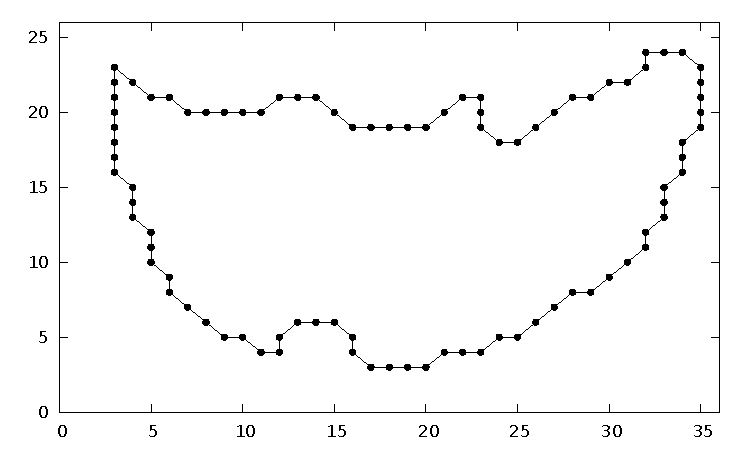
\includegraphics[width=0.45\textwidth]{fig/curva} }
        \subfigure[Curva aproximada]
        {
            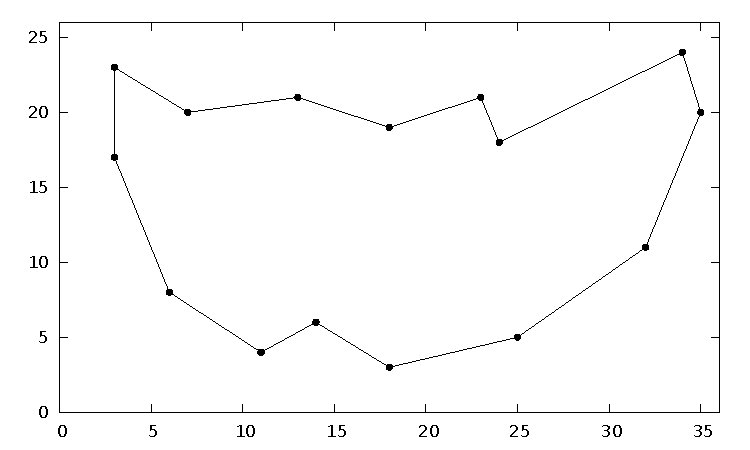
\includegraphics[width=0.45\textwidth]{fig/curva_aproximada}
        }
    \end{figure}
}

\section{Caminhos mínimos}
\stepcounter{subsection}

\framet[Caminhos mínimos]{
  Definições:
  \begin{itemize}
    \pause \item \defi{função custo} $c$ para todo $uv \in A$, $c(uv)$ é 
      o custo do arco $uv$;
    \pause \item \defi{custo do caminho} $P$, $c(P) = 
      \displaystyle\sum_{uv \in P}{c(uv)}$;
    \pause \item caminho $P$ de \defi{custo mínimo}, para qualquer 
      caminho $Q$ de mesma origem e destino vale $c(P) \leq c(Q)$;
    \pause \item \defi{distância} de dois vértice $\scor$ a $\tcor$, 
      $\dist{\scor,\tcor}$;
    \pause \item \defi{maior custo} de um arco, $C = \max\{c(uv) \tq uv 
      \in A \}$.
  \end{itemize}
}


\framet[Caminhos mínimos]{
  \begin{problema}{\spp$(G,c,\scor,\tcor)$} Como parâmetros do problema 
    são dados
    \begin{itemize}
      \item\ um grafo direcionado $G = (V, A)$,
      \item\ uma função custo $c$ sobre $G$,
      \item\ um vértice origem $\scor$ e
      \item\ um vértice destino $\tcor$.
    \end{itemize}

    O problema consiste em encontrar um caminho de custo mínimo de $\scor$ a 
    $\tcor$.
  \end{problema}


}

\framei[Caminhos mínimos]{
  \footnotesize
\pause \item Vamos definir o seguinte programa linear primal: encontrar 
  um vetor $x$ indexado por $A$ que
  \begin{linearprogram}
    \mbox{minimize}
    & \displaystyle\sum_{uv \in A} c(uv)x_{uv} \\
    \mbox{sob as restrições}
    &\displaystyle\sum_{vw \in A}{x_{vw}} - \displaystyle\sum_{uv \in 
  A}{x_{uv}} &=& \left\{ \begin{array}{rl}
           1 & \text{para } v = \scor\\
           0 & \text{para todo } v \in V \setminus \{\scor, \tcor\} \\
          -1 & \text{para } v = \tcor\\
          \end{array} \right. & \\
                              & x_{uv} & \geq & 0\ \text{ para todo } uv 
                       \in A. & 

  \end{linearprogram}

\pause \item Vamos definir agora, o respectivo problema dual, que 
  consiste em encontrar um vetor $y$ indexado por $V$ que
  \begin{linearprogram}
    \mbox{maximize} & y(\tcor)-y(\scor) \\
\mbox{sob as restrições} & y(v) -  y(u) & \leq & c(uv) &
    \mbox{para todo $uv \in A$.}
  \end{linearprogram}
}

\framei[Caminhos mínimos]{
\pause \item Uma \textbf{função-potencial} é uma função sobre $V$ que 
  associa a cada vértice um valor.
\pause \item Se $y$ é uma função potencial e $c$ é uma função custo, 
  então, dizemos que $y$ é um \defi{$c$-potencial} se \begin{center}
  $y(v) - y(u) \leq c(uv)$ para cada arco $uv \in A$.
\end{center}
\pause \item A partir de uma função-potencial podemos extrair um 
  \defi{certificado de otimalidade} ou um \defi{certificado de não 
  acessibilidade} (ver \citet{pf:proglin}).
}

\framei[Caminhos mínimos]{
\pause \item Representação de caminhos:
  \begin{itemize}
  \footnotesize
    \item Uma \textbf{função predecessor} $\pred$ é uma função sobre $V$ 
      tal que, para cada $v$ em $V$,
      \[
        \pred(v) = \nil \quad \mbox{ou} \quad (\pred(v),v) \in A\mbox{.} 
      \]
  %\footnotesize
    %\item Dados um grafo direcionado $G = (V,A)$, uma função 
    %predecessor $\pred$ sobre $V$ e um caminho $P = \seq{v_{0}, v_{1}, 
    %\ldots,v_{k}}$, dizemos que $P$ é um \textbf{caminho determinado 
    %por $\pred$} se
%$$ v_{0} = \pred(v_{1}), v_{1} = \pred(v_{2}),
%\ldots, v_{k-1} = \pred(v_{k})\mbox{.}$$

\end{itemize}
\pause \item Examinando arcos e vértices:
  \begin{itemize}
  \footnotesize
    \item \defi{Examinar um arco} ou \defi{relaxar/rotular um arco} 
      (\textit{relaxing}~\cite{clrs:introalg-2001}, \textit{labeling 
      step}~\cite{tarjan:data}) é uma operação que envolve $\pred$ e 
      $y$, e consiste em verificar se $y$ respeita $c$ em $uv$ e, caso 
      não respeite ($y(v) - y(u) > c(uv)$) fazer \[
  y(v) \larr y(u) + c(uv) \ \ \mbox{e} \ \ \pred(v) \larr u\mbox{.}
\]
\end{itemize}
}

\framei[Caminhos mínimos]{
\item O algoritmo de Edsger Wybe Dijkstra~\citep{dijkstra:59} resolve o 
  problema do caminho mínimo se $c(uv) \geq 0$ para todo $uv \in A$
  (para detalhes \citet{fabio:09} e \citet{pf:fluxos}).
  \begin{itemize}
    \pause \item O algoritmo é iterativo. No início de cada iteração 
      tem-se os conjuntos $S$ e $Q$ ($S \cap Q = \emptyset$ e $S \cup Q 
      = V$).
  \pause \item O algoritmo conhece caminhos de custo mínimo partindo de 
  $\scor$ a cada vértice em $S$, caminhos estes que são garantidamente 
de custo mínimo, e conhece caminhos a uma parte dos vértices em $Q$.  
\pause \item Antes da primeira iteração temos $S = \emptyset$ e $Q = V$.  
\pause \item Cada iteração consiste em retirar um determinado vértice de 
  $Q$, examiná-lo e adicioná-lo a $S$.
\pause \item Se o conjunto $Q$ é vazio podemos parar o processamento.
  \end{itemize}
}

\framet[Caminhos mínimos]{
  \footnotesize
  \begin{algoritmo}
    \Dijkstra{} $(V, A, c, \scor)$

    \d1\x \para{} \cada{} $v$ em $V$ \textbf{faça}

    \d2\xx    $y(v) \larr nC+1$

    \d3\xx    $\pred(v) \larr \nil$

    \d4\x  $y(\scor) \larr 0$

    \d5\x $Q \larr V$

    \d6\x \enquanto{} $Q \neq \seq{}$ \textbf{faça}

    \d7\xx retire de $Q$ um vértice $u$ com $y(u)$ mínimo

    \d8\xx \para{} \cada{} $uv$ em $A$ \textbf{faça}

    \d9\xxx \se{} $y(v) > y(u) + c(uv)$ \textbf{então}

    10\xxxx $y(v) \larr y(u)+ c(uv) $

    11\xxxx $\pred(v) \larr u$

    12\x \devolva{} $\pred$ e $y$
  \end{algoritmo}
}

\framei[Caminhos mínimos]{
\item O algoritmo proposto por Ford \citep{bellman:58}, pode ser 
  aplicado a grafos cujos arcos têm custos negativos, que não possuem 
  circuitos de custo negativo \citep{carlos:98}.
  \begin{itemize}
    \pause \item Este algoritmo consiste em examinar os vértices do 
      grafo, corrigindo os potenciais tantas vezes quantas forem 
      necessárias, até que todos os potenciais satisfaçam a condição de 
      otimalidade.
    \pause \item Diferentemente do algoritmo de \Dijkstra, os potenciais só 
  se tornam definitivos após terminar a execução do algoritmo.
  \end{itemize}
}

\framet[Caminhos mínimos]{
  \footnotesize
\begin{algoritmo}
  \Ford{} $(V, A, c, \scor)$ \quad {$\rhd$  $(V, A, c)$ não possui 
  ciclos negativos}

  1\x \para{} \cada{} $v$ em $V$ \textbf{faça}

  2\xx    $y(v) \larr nC+1$ \quad {$\rhd$  $nC+1$ faz o papel de 
  $\infty$} 

  3\xx    $\pred(v) \larr \nil$

  4\x  $y(\scor) \larr 0$

  5\x \enquanto{} $y(v) > y(u) + c(uv)$ \para~{\bf algum} $uv \in A$ 
  \textbf{faça}

  6 \xx $y(v) \larr y(u) + c(uv)$ 

  7 \xx $\pred(v) \larr u$

  8\x \devolva{} $\pred$ e $y$
\end{algoritmo}


}

\section{Caminhos mínimos com recursos limitados}
\stepcounter{subsection}

\framet[Definição formal do problema]{
\tiny
  \pause \begin{problema}{\rcsp($G, \scor, \tcor, k, r, \lambda, c$)} 
    Como parâmetros do problema são dados
    \begin{itemize}
  \tiny
      \item\ um grafo direcionado $G=(V,A)$,
      \item\ um vértice origem $\scor \in V$ e um vértice destino $\tcor 
        \in V$, $\scor \neq \tcor$,
      \item\ um número $k \in \mathbb{N}$ de recursos disponíveis 
        $\{1,\dots,k\}$,
      \item\ o consumo de recursos $r^i_{uv} \in \mathbb{N}_0$ de cada 
        arco de $G$ sobre os  $k$ recursos disponíveis, $i = 1, \dots, 
        k$, $uv \in A$,
      \item\ o limite $\lambda^i \in \mathbb{N}_0$ que dispomos de cada 
        recurso, $i = 1, \dots, k$,
      \item\ o custo $c_{uv} \in \mathbb{N}_0$, para cada arco, $uv \in 
        A$.
    \end{itemize}

    \pause O consumo de um recurso $i$, $i = 1, \dots, k$ em um 
    $st$-caminho $P$ é $r^i(P) = \sum_{uv \in P}{r^i_{uv}}$. Um 
    $st$-caminho $P$ é limitado pelos recursos $1, \dots, k$ se $ r^i(P) 
    \leq \lambda^i$, $i = 1, \dots, k$.
    O custo de um $st$-caminho $P$ é $c(P) = \sum_{uv \in P}{c_{uv}}$.
    O problema \rcsp\ consiste em encontrar o caminho limitado pelos 
    recursos de
    menor custo.

  \end{problema}

  \pause Usamos $n = |V|$ e $m = |A|$. Quando
  se tratando de um contexto onde existe apenas um recurso usamos apenas 
  $\lambda$ para representar $\lambda^1$ e apenas $r_{uv}$ para 
  representar $r^1_{uv}$. 

}

\framet[Algumas publicações relevantes]{
  \tiny
\begin{table}[ht!]
\centering
\begin{tabular}{|c|c|c|c|c|}
  \hline
  Referencia & Versão do \rcsp &  Método & Custo & Grafo\\
  \hline
  \citet{zang:80} & único recurso & \textsc{RL} + \textsc{Yen} & $c_{uv} 
          \geq 0$ & gerais\\
  \hline
  \citet{beasley:89} & múltiplos recursos & \textsc{RL} + \textsc{BB} & irrestrito & gerais\\
  \hline
  \citet{mehlhorn:00} & múltiplos recursos & \textsc{PL} & $c_{uv} \geq 0$ & gerais\\
  \hline
  \citet{joksch:66} & único recurso & \textsc{PD} & $c_{uv} > 0$ & gerais\\
  \hline
  \citet{aneja:83} & múltiplos recursos & \textsc{LS} & $c_{uv} \geq 0$ & gerais\\
  \hline
  \citet{hassin:92} & único recurso & \textsc{PD} & $c_{uv} > 0$ & acíclicos\\
  \hline
  \citet{dumitrescu:03} & múltiplos recursos & \textsc{LS} & $c_{uv} 
                \geq 0$ & gerais\\
  \hline
\end{tabular}
\caption{\tiny Principais algoritmos disponíveis para o \rcsp.}
\textsc{RL} -- relaxação lagrangiana; \textsc{KSP} -- $k$-ésimo menor 
caminho; \textsc{BB} -- \emph{branch and bound}; \textsc{PL} -- 
relaxação linear; \textsc{PD} -- programação dinâmica; \textsc{LS} -- 
rotulamento permanente.
\label{tab:algs}
\end{table}


}

\framei[Complexidade]{
  \footnotesize
\pause \item \citet{zang:80, jaffe:84} mostraram que o \rcsp~é 
  $\mathcal{NP}$-difícil, mesmo em grafos acíclicos, com restrições 
  sobre um único recurso, e com todos os consumos de recursos positivos 
  \citep{dumitrescu:03}.
\pause \item \citet{garey:79} apresentaram uma redução do problema da 
  partição para o \rcsp, enquanto \citet{zang:80} reduziu o problema da 
  mochila para o nosso problema.
\pause \item \citet{hassin:92} mostrou que o \srcsp~ tem solução 
  polinomial se os custos dos arcos e consumos de recursos são 
  limitados.
}

\framet[Problema da mochila]{
  \footnotesize
\begin{problema}{\textsc{Mochila}(N,w,v,D)}
Como parâmetros do problema são dados:
\begin{itemize}
\item\ um conjunto de itens $N = \{1, \dots, n\}$,
\item\ pesos $w_i \in \mathbb{N}$, $i = 1, \dots, n$, para esses itens,
\item\ valores $v_i \in \mathbb{N}$, $i = 1, \dots, n$, para esse itens,
\item\ um peso limite $D \in \mathbb{N}_0$.
\end{itemize}
\pause O peso de um subconjunto $I \subseteq N$ é
$w(I) = \sum_{i \in I}{w_i}$, e seu valor é 
$v(I) = \sum_{i \in I}{v_i}$. O problema \textsc{Mochila} consiste em
encontrar um subconjunto de itens com valor máximo, cujo peso não excede
o limite $D$.
\end{problema}
}

\framet[Redução \mochila~ para \rcsp]{
\begin{itemize}
    \tiny
\item $V = N \cup \{0\}$.
\item Entre cada par de vértice $i-1$ e $i$, onde $i = 1, 2, \cdots, n$,  
  teremos duas arestas paralelas $(i-1, i)$ que estarão separadas, uma 
  em cada um dos dois subconjuntos $A_1$ e $A_2$ que compõem $A$.  
  \begin{itemize}
    \tiny
        \item $A = A_1 \cup A_2$,
        \item $A_1 = \{(i-1,i): i=1,\dots,n\}$,
        \item $A_2 = \{(i-1,i): i=1,\dots,n\}$.
    \end{itemize}
\item $
r_{uv} = \left\{
  \begin{array}{ll}
		\begin{array}{ll}
      w_i, & \mbox{se } uv \in A_1, \\
			0, & \mbox{caso contrário}
    \end{array} & \mbox{para todo } uv \in A.
	\end{array}
	\right.
$
\item
$
c_{uv} = \left\{
  \begin{array}{ll}
    \begin{array}{ll}
      M - v_i, & \mbox{se } {uv} \in A_1, \\
      M, & \mbox{caso contrário}
    \end{array} & \mbox{para todo } {uv} \in A.
	\end{array}
	\right.
$
\item $\scor = 0$.
\item $\tcor = n$.
\item $k = 1$.
\item $\lambda = D$.

\end{itemize}


}

\framet[Grafo gerado pela redução]{
\begin{figure}[h!]
  \centering
  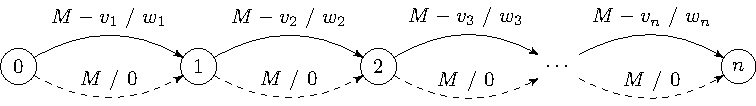
\includegraphics[scale=0.8]{fig/reducao_mochila}
  \caption[\tiny Grafo da redução do problema \textsc{Mochila} para o 
  problema \rcsp]{ Os arcos contínuos representam os arcos no conjunto 
    $A_1$ e os arcos tracejados representam os arcos no conjunto $A_2$.  
    O rótulo de cada arco $uv$ representa o seu custo e o seu consumo de 
  recurso, respectivamente ($c_{uv}$ / $r_{uv}$).}
  \label{fig:rscp_mochila}
\end{figure}


}

\framet[Prova da redução]{
  \tiny
\pause \begin{equation}
\begin{array}{rcl}
c(P) & = & \displaystyle\sum_{a^1_i \in X}{(M-v_i)} + 
  \displaystyle\sum_{a^2_i \in Y}{M}\\
     & = & n \cdot M - \displaystyle\sum_{a^1_i \in X}{v_i}\\
     & = & n \cdot M - v(S)
\end{array}
\label{eq:reducao_custo}
\end{equation}

\pause \begin{equation}
\begin{array}{rcl}
r(P) & = & \displaystyle\sum_{a^1_i \in X}{w_i} + 
  \displaystyle\sum_{a^2_i \in Y}{0} \\
     & = & \displaystyle\sum_{a^1_i \in X}{w_i} \\
     & = & w(S)
\end{array}
\label{eq:reducao_recurso}
\end{equation}

\pause \begin{displaymath}
\begin{array}{rcl}
r(P) \leq \lambda & \Longleftrightarrow & w(S) \le D$$\\
\mbox{ minimizar } c(P) & \Longleftrightarrow & \mbox{ maximizar }v(S)
\end{array}
\end{displaymath}
\

}

\framei[Preprocessamento]{
  \tiny
\pause \item Redução baseada nos recursos:

Denotamos por $R_{uv}$ a menor quantidade de recurso que podemos usar do 
vértice $u$ até o vértice $v$. Qualquer vértice $v$ para o qual vale que 
$$ R_{\scor v} + R_{v \tcor} > \lambda$$ pode ser removido do grafo 
(este vértice não pode pertencer a qualquer caminho viável). De forma 
similar, qualquer arco $uv$ para o qual vale que $$ R_{\scor u} + r_{uv} 
+ R_{v \tcor} > \lambda$$ pode ser removido do grafo.

\pause \item Redução baseada nos custos:

Para um limite superior $UB$ conhecido para o problema, nós podemos 
estender a ideia para uma redução baseada em custos. Denotamos por 
$C_{uv}$ o menor custo para um caminho de $u$ até $v$. Um vértice $v$ 
para o qual vale que $$C_{\scor v} + C_{v \tcor} > UB$$ pode ser 
removido, da mesma forma que um arco $uv$ para o qual vale que 
$$C_{\scor u} + c_{uv} + C_{v \tcor} > UB$$ pode ser removido.
}

\framei[Programação dinâmica primal]{
  \footnotesize
\pause \item Descrita primeiramente por \citet{joksch:66} (ver também 
  \citet{goldman:65, lawler:76}).
\pause \item Definimos $f_v(r)$ como sendo o menor custo possível para 
  um caminho de $\scor$ a $v$, que consome no máximo $r$ unidades de 
  recurso, e assim temos:
\begin{displaymath}
f_v(r) = \left\{
\begin{array}{lcl}
0, & &\text{se } v=\scor  \\ & & \text{ e } r=0,\dots,\lambda\\
 & & \\
\infty, & & \text{se } v\neq \scor  \\ & & \text{ e } r=0\\
 & & \\
\min\left\{f_v(r-1), \displaystyle\min_{u|r_{uv}\leq 
r}\{f(r-r_{uv})+c_{uv}\}\right\}, & & \text{se } v\neq \scor  \\ & & \text{ 
  e } r=1,\dots,\lambda\\
\end{array}
\right.
\end{displaymath}

}

\framet[Programação dinâmica primal]{
  \tiny
  \begin{algoritmo}
    \textsc{Programação-Dinâmica-Primal} $(\tcor, \lambda)$

    \d1\x $\pd \larr [~]$ \quad {$\rhd$ tabela de programação dinâmica}

    \d2\x \para{} \cada{} $r$ em $\{0,1,\cdots,\lambda\}$ \textbf{faça}

    \d3\xx $\pred(\scor,r) \larr \nil$

    \d4\xx $\pd[\scor,r] \larr 0$

    \d5\x \para{} \cada{} $v$ em $V \setminus \{\scor\}$ \textbf{faça}

    \d6\xx $\pred(v,0) \larr \nil$

    \d7\xx $\pd[v,0] \larr \infty$

    \d8\x \para{} $r$ de $1$ até $\lambda$ \textbf{faça}

    \d9\xx    \para{} \cada{} $v$ em $V \setminus \{\scor\}$ 
    \textbf{faça}

    10\xxx       $\pred(v,r) \larr \pred(v,r-1)$

    11\xxx       $\pd[v,r] \larr \pd[v,r-1]$

    12\xxx       \para{} \cada{} $uv$ em $A$ \textbf{faça}

    13\xxxx          \se{} $r_{uv} \leq r$ \textbf{então}

    14\xxxxx              \se{} $\pd[v,r]>\pd[v,r-r_{uv}]+c_{uv}$ 
    \textbf{então}

    15\xxxxxx                 $\pred(v,r) \larr u$

    16\xxxxxx                 $\pd[v,r] \larr \pd[v,r-r_{uv}]+c_{uv}$

    17\x \devolva{} $\pd[\tcor, \lambda]$
  \end{algoritmo}
}

\framei[Programação dinâmica dual]{
  \footnotesize
  \pause \item Descrito por \citet{hassin:92}.
  \pause \item Digamos que $g_v(c)$ denota o menor consumo de recursos 
    possível para um caminho de $\scor$ a $v$ que custa no máximo $c$.  
    Então a seguinte recorrência pode ser definida.
    \tiny
\begin{displaymath}
g_v(c) = \left\{
\begin{array}{lcl}
0, & &\text{se } v=\scor \\ & &  \text{ e } c=0,\dots,OPT\\
 & & \\
\infty, & & \text{se } v\neq \scor \\ & & \text{ e } c=0\\
 & & \\
\min\left\{g_v(c-1), \displaystyle\min_{u|c_{uv}\leq c}\{g(c-c_{uv})+r_{uv}\}\right\}, & & \text{se } v\neq \scor \\ & & \text{ e } c=1,\dots,OPT\\
\end{array}
\right.
\end{displaymath}

 }

\framet[Programação dinâmica dual]{
  \tiny
\begin{algoritmo}
  \textsc{Programação-Dinâmica-Dual} $(\tcor, \lambda)$

  \d1\x $\pd \larr [~]$ \quad {$\rhd$ tabela de programação dinâmica}

  \d2\x $\pred(\scor,0) \larr \nil$

  \d3\x $\pd[\scor,0] \larr 0$

  \d4\x \para{} \cada{} $v$ em $V \setminus \{\scor\}$ \textbf{faça}

  \d5\xx    $\pred(v,0) \larr \nil$

  \d6\xx    $\pd[v,0] \larr \infty$

  \d7\x $c \larr 0$

  \d8\x \enquanto{} $\pd[\tcor, c] > \lambda$ \textbf{faça}

  \d9\xx    $c \larr c + 1$

  10\xx     $\pred(\scor,c) \larr \nil$

  11\xx     $\pd[\scor,c] \larr 0$

  12\xx     \para{} \cada{} $v$ em $V \setminus \{\scor\}$ \textbf{faça}

  13\xxx       $\pred(v,c) \larr \pred(v,c-1)$

  14\xxx       $\pd[v,c] \larr \pd[v,c-1]$

  15\xxx       \para{} \cada{} $uv$ em $A$ \textbf{faça}

  16\xxxx          \se{} $c_{uv} \leq c$ \textbf{então}

  17\xxxxx              \se{} $\pd[v,c]>\pd[v,c-c_{uv}]+r_{uv}$ 
  \textbf{então}

  18\xxxxxx                 $\pred(v,c) \larr u$

  19\xxxxxx                 $\pd[v,c] \larr \pd[v,c-c_{uv}]+r_{uv}$

  20\x $OPT \larr c$

  21\x \devolva{} $OPT$, $\pd[\tcor, OPT]$
\end{algoritmo}

}

\framet[Relaxação Lagrangiana]{
  \footnotesize
\pause Algoritmo proposto por \citet{zang:80}. Se utiliza de uma 
relaxação da formulação abaixo para o problema usando programação linear 
(problema \textbf{(P)}).  \begin{linearprogram}
\mbox{minimize}
  & c(x) & = & \displaystyle\sum_{uv \in A} c_{uv}x_{uv} \\
\mbox{sob as restrições}
  &\displaystyle\sum_{vw \in A}{x_{vw}} - \displaystyle\sum_{uv \in 
  A}{x_{uv}} &=& \left\{ \begin{array}{rl}
               1, & \text{para } v = \scor\\
               0, & \text{para todo } v \in V \setminus \{\scor, 
               \tcor\}\\
              -1, & \text{para } v = \tcor\\
          \end{array} \right. & (1)\\
      &\displaystyle\sum_{uv \in A} r_{uv}x_{uv} &\le& \lambda & (2)\\
      & x_{uv} & \in & \{0,1\},\ uv \in A & (3)
\end{linearprogram}
\pause \begin{itemize}
  \item Vamos denotar por $\cal{X}$ o conjunto de vetores $x$ que contêm 
    um caminho de $\scor$ a $\tcor$ e definir a função $g(x) = 
    \displaystyle\sum_{uv \in A}{r_{uv} x_{uv}} - \lambda$.
\end{itemize}
\pause
$$c^* = c(x^*) = min \left\{\ c(x) \mid x \in {\cal{X}} \mbox{ e } g(x) 
\leq 0\ \right\} $$
}

\framet[Relaxação Lagrangiana]{
  \footnotesize
\pause Para qualquer $u \in \mathbb{R}$, definimos a função
lagrangiana.
$$L(u) = \displaystyle\min_{x \in \cal{X}}{L(u,x)} \text{, onde }
L(u,x) = c(x) + u g(x)$$

\pause Temos que $L(u) \leq c^*$ para qualquer $u \geq 0$ pois
$$ g(x^*) \leq 0 \Rightarrow L(u) \leq c(x^*) + u g(x^*) \leq c(x^*) = 
c^* \text{,}$$
o que nos permite usar $L(u)$ como um \textbf{limite inferior} para
o problema original.

\pause Para encontrarmos o limite inferior mais justo
possível, resolvemos o problema \textbf{(D)} a seguir.

\begin{linearprogram}
	& L^* = L(u^*) = \displaystyle\max_{u \geq 0}{L(u)} \hfill &&&
\end{linearprogram}

}

\framet[Relaxação Lagrangiana]{
  {\footnotesize Vamos descrever um método para
resolver o problema. Por praticidade vamos denotar por $x(u)$ como um 
caminho que possui valor ótimo associado à função $L(u)$. }

\pause \begin{itemize}
  \item Passo $1$
\begin{itemize}
\item Se $g(x(0)) \leq 0$, então $x(0)$ é claramente uma solução ótima 
  de $(P)$.
\item Senão, $x(0)$ nos serve, pelo menos, como limite inferior para a 
  solução.
\end{itemize}

\pause  \item Passo $2$
\begin{itemize}
\item Se $g(x(\infty)) > 0$, o problema não tem solução, pois o consumo 
  do caminho que consome a menor quantidade de recursos ultrapassa o 
  limite dado.
\item Senão, $x(\infty)$ é uma solução viável para a instância e nos serve de
limite superior para o problema.
\end{itemize}

\end{itemize}
}


\framei[Relaxação Lagrangiana]{
\pause \item Temos a seguinte situação:
Dois caminhos, $x(0)$, que {\bf não é solução} e é um {\bf limite 
inferior} e $x(\infty)$,
que {\bf é solução viável} e é um {\bf limite superior}, $g(x(0)) > 0$ e 
$g(x(\infty)) \leq 0$.
\pause \item Podemos interpretar cada caminho no grafo como
uma reta no espaço $(u,L)$ da forma  $L = c(x) + u g(x)$.
%\item Como estamos procurando o valor
%de $L^*$ (o ponto ``mais alto'' da função $L(u)$) vamos analisar o ponto 
%$(u',L')$ que é a intersecção
%das retas associadas a $x(0)$ e $x(\infty)$. 
%$$u' = (c(x(\infty)) - c(x(0))) / (g(x(0)) - g(x(\infty)))$$ 
%$$L' = c(x(0)) + u' \cdot g(x(0))$$
}

\framei[Relaxação Lagrangiana]{
\item Passo $3$
  \begin{itemize}
    \pause \item Temos dois caminhos disponíveis $x^+,x^- \in \cal{X}$
    \pause \item $g^+ \equiv g(x^+) > 0$, $g^- \equiv g(x^-) \leq 0$ e 
      $c^- \equiv c(x^-) \geq c^+ \equiv c(x^+)$.
    \pause \item $u' = (c^- - c^+) / (g^+ - g^-)$ e $L' = c^+ + u'g^+$ 
      definem o ponto de intersecção, no espaço $(u,L)$, das retas 
      associadas aos caminhos $x^+$ e $x^-$.
      \begin{itemize}
        \pause \item se $L(u') = L'$ ou se $g(x(u')) = 0$, então $L(u^*) 
          = L(u')$ é a solução do nosso
        problema dual $(D)$;
      \pause \item se $g(x(u')) < 0$, então $x(u')$ é o nosso novo
      caminho $x^-$, e
    \pause \item se $g(x(u')) > 0$, então $x(u')$ é o nosso novo caminho 
      $x^+$.
      \end{itemize}
  \end{itemize}
}

\framei[Relaxação Lagrangiana]{
\pause \item Ao final do procedimento temos disponíveis um limite 
  inferior $LB$ ({\it lower bound})
e um limite superior $UB$ ({\it upper bound}) para o valor de $c^*$.
\pause \item $LB = L(u^*) \leq c(x^*)$ pelo teorema fraco da dualidade;
\pause \item  $UB$ é o valor do menor $c^-$ calculado no procedimento.

\pause \item Quando $LB = UB$, a solução associada a $LB$ é ótima.
Porém, quando $LB < UB$ temos um folga na dualidade. 

\pause \item Para eliminarmos essa folga usamos um algoritmo de 
  $k$-ésimo menor caminho ({\it k-shortest path}) em relação à função 
  lagrangiana $L(u^*,x)$ (o que é equivalente a  usar a função $c'$ como 
  custo, $c'_{uv} = c_{uv} + u^* \cdot r_{uv}$, $uv \in A$).
}

\framet[Relaxação Lagrangiana]{
\begin{figure}[ht!]
    \centering
        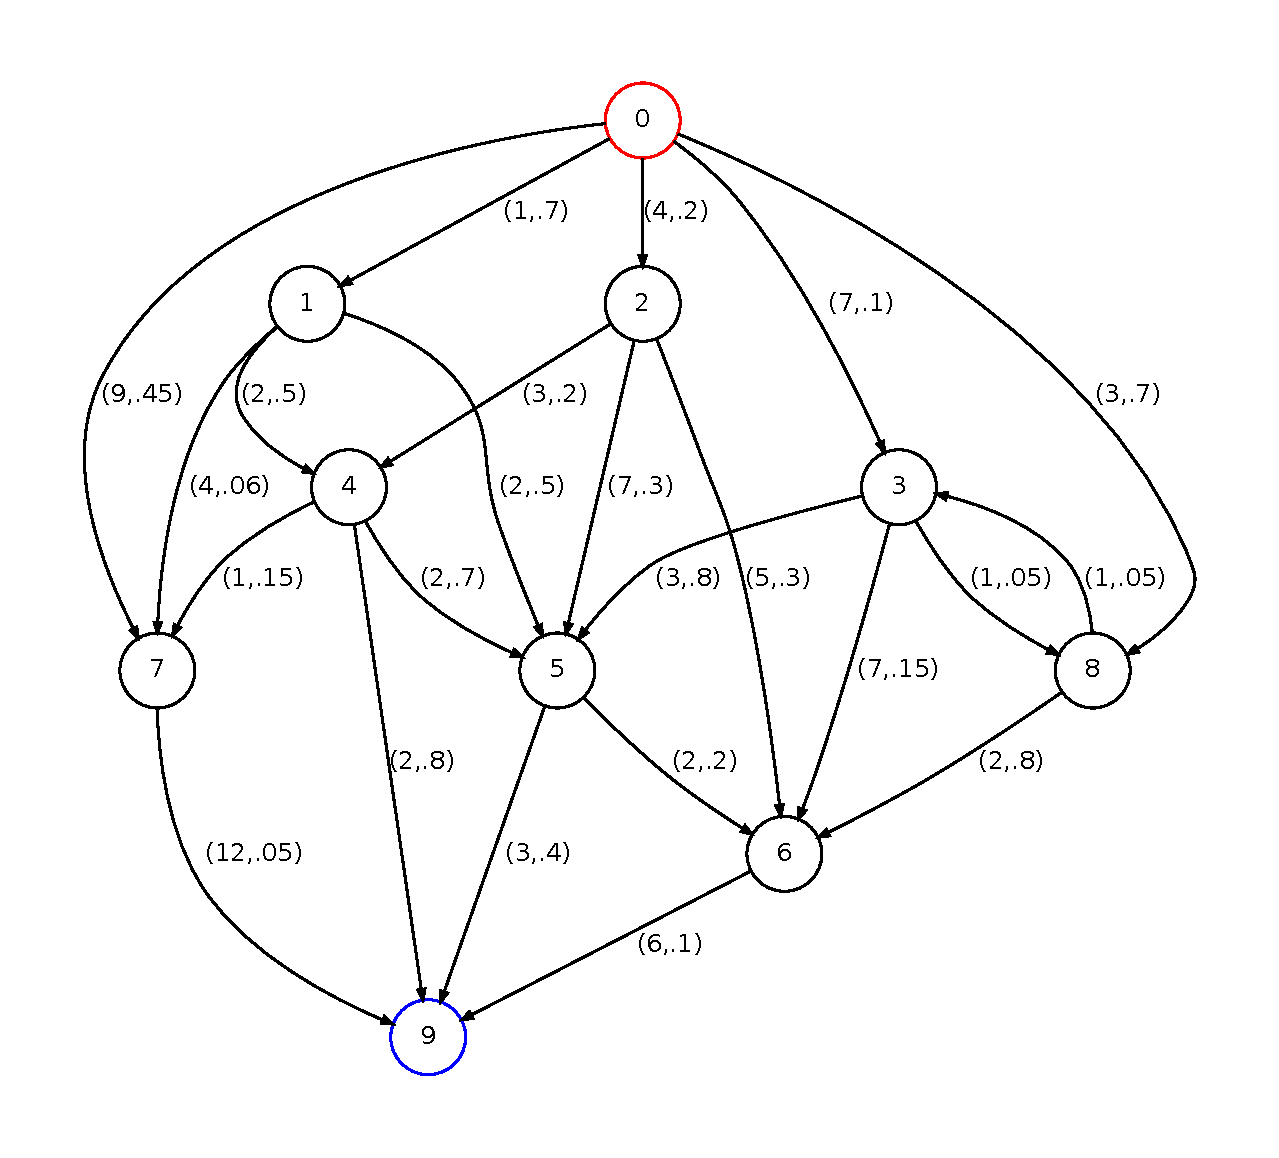
\includegraphics[scale=0.25]{fig/grafo_lagrangeana.pdf}
    \caption{\tiny\it Grafo exemplo; os rótulos dos arcos representam 
    $(c_{uv}, r_{uv})$. }
    \label{fig:exemplo_grafo}
\end{figure}
}
\framet[Relaxação Lagrangiana]{

\begin{figure}[h!]
  \centering
  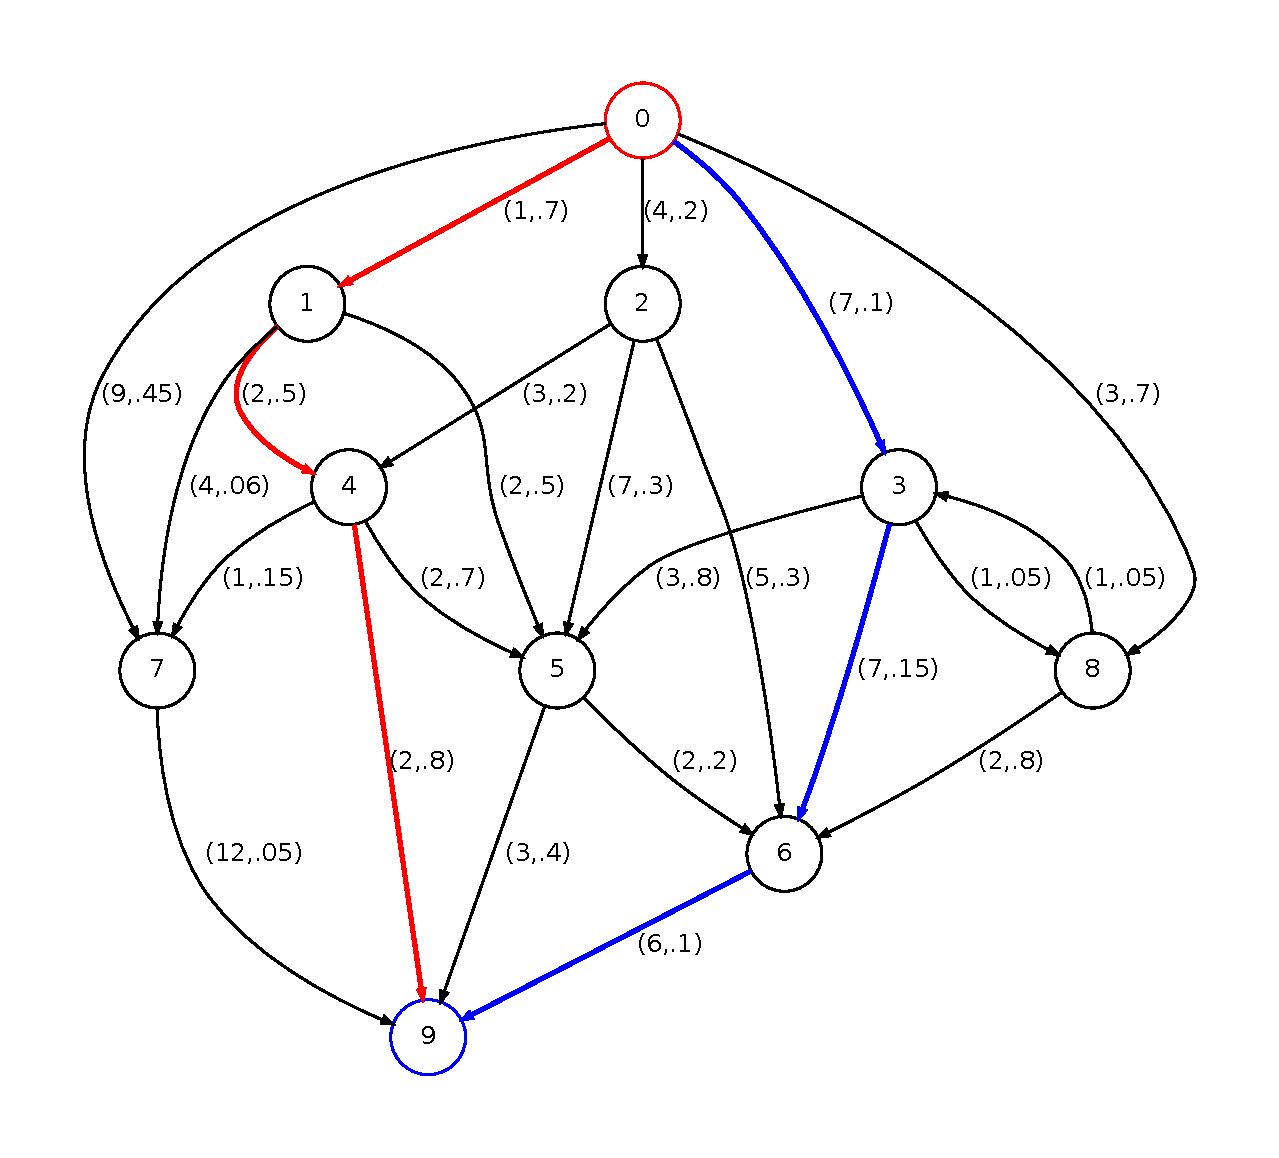
\includegraphics[scale=0.25]{fig/zang1a.pdf}
  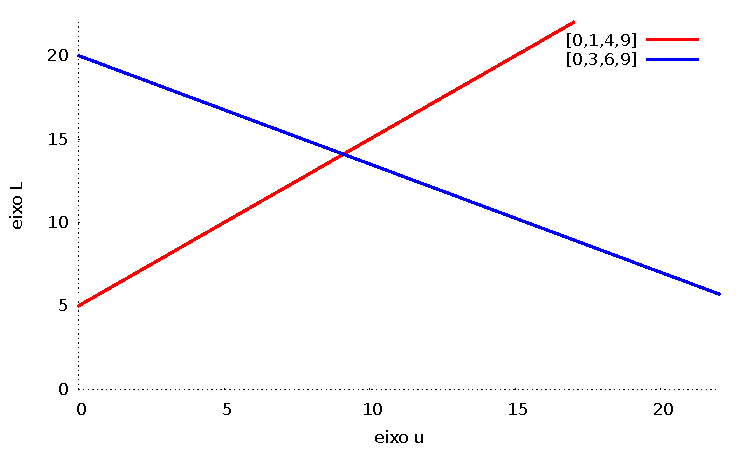
\includegraphics[scale=0.5]{fig/zang1b.pdf}
  \caption[Exemplo do algoritmo de Handler e Zang]{\tiny Inicialmente 
    encontramos $x_0=[0,1,4,9]$ e $x_{\infty}=[0,3,6,9]$. As restas 
    correspondentes são $L=5+u$ e $L=20-0.65u$ que se intersectam no 
    ponto $u' = 9.09$ e $L'=14.09$. Nesta primeira iteração temos $LB = 
  5$ e $UB = 20$.}
  \label{fig:zang1}
\end{figure}
}
\framet[Relaxação Lagrangiana]{
\begin{figure}[h!]
  \centering
  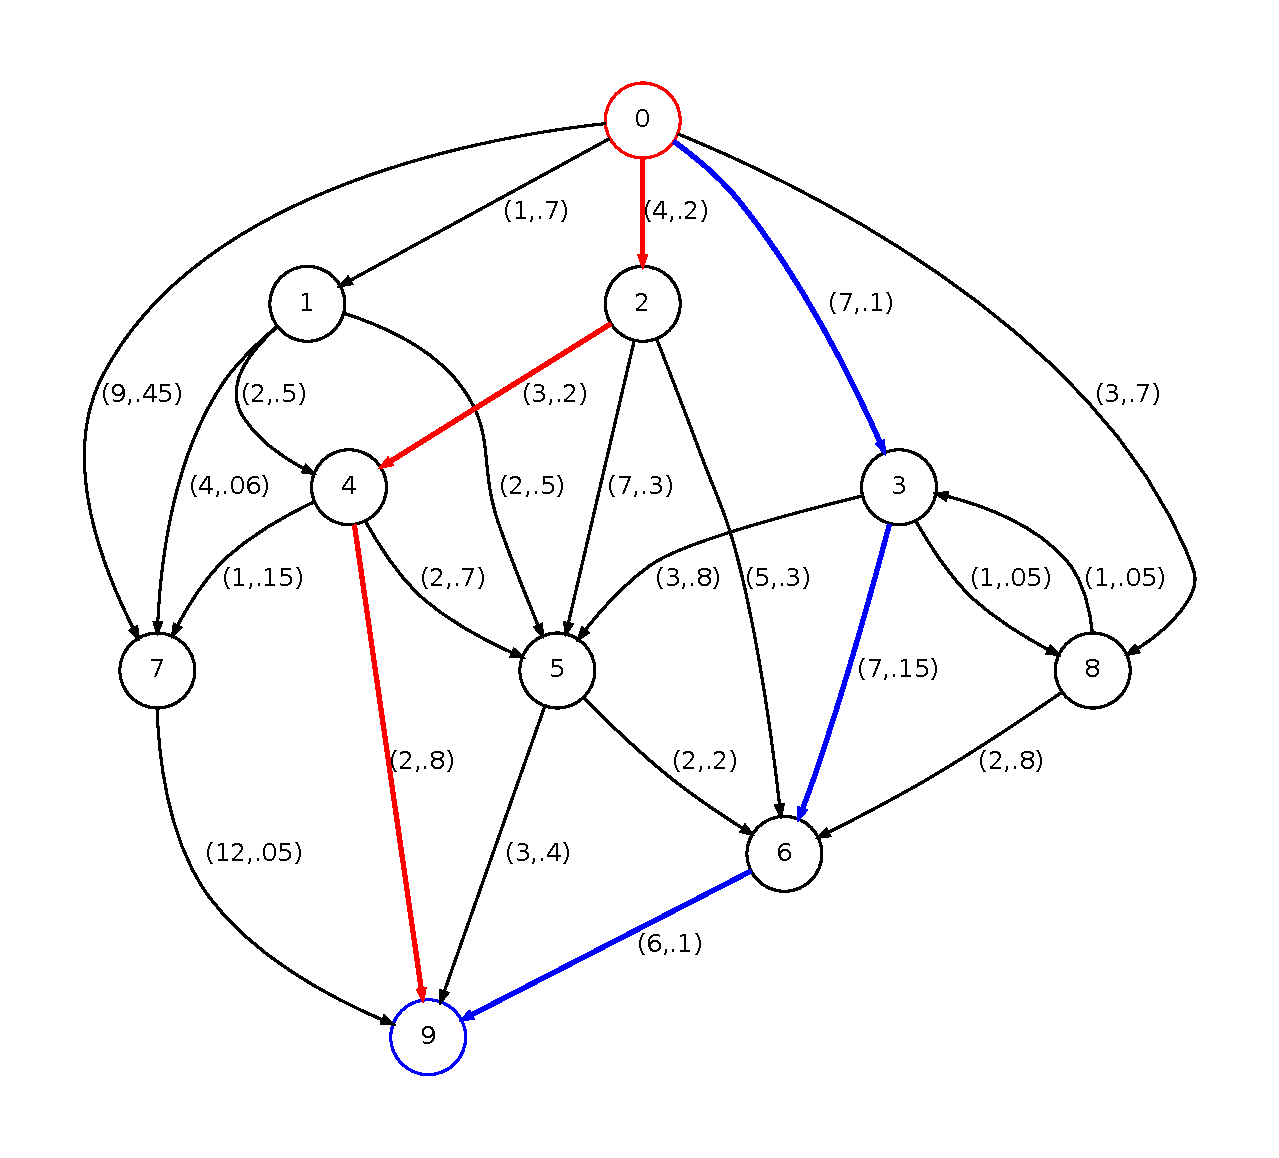
\includegraphics[scale=0.25]{fig/zang2a.pdf}
  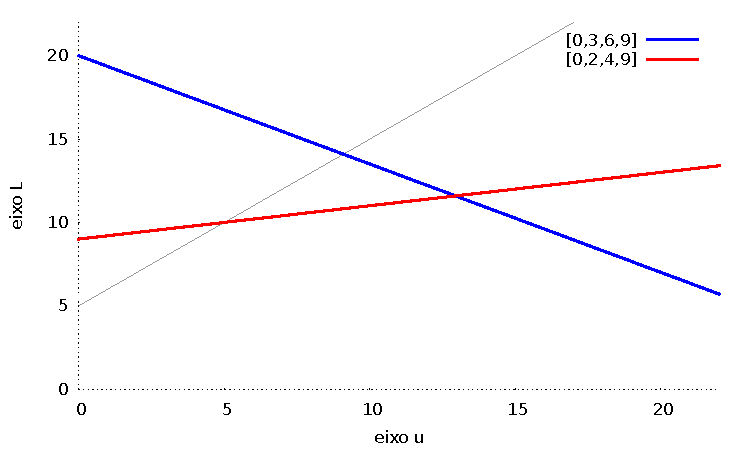
\includegraphics[scale=0.5]{fig/zang2b.pdf}
  \caption[Exemplo do algoritmo de Handler e Zang]{\tiny Calculando a 
    função $L$ no ponto $u'$ encontramos um novo caminho para $x^+$ que 
    passar a ser $[0,2,4,9]$.  Temos agora $LB = 10.8$ e $UB = 20$. A 
    interseção das restas é sobre o ponto $u' = 12.94$ e $L' = 11.59$.}
  \label{fig:zang1}
\end{figure}
}
\framet[Relaxação Lagrangiana]{
\begin{figure}[h!]
  \centering
  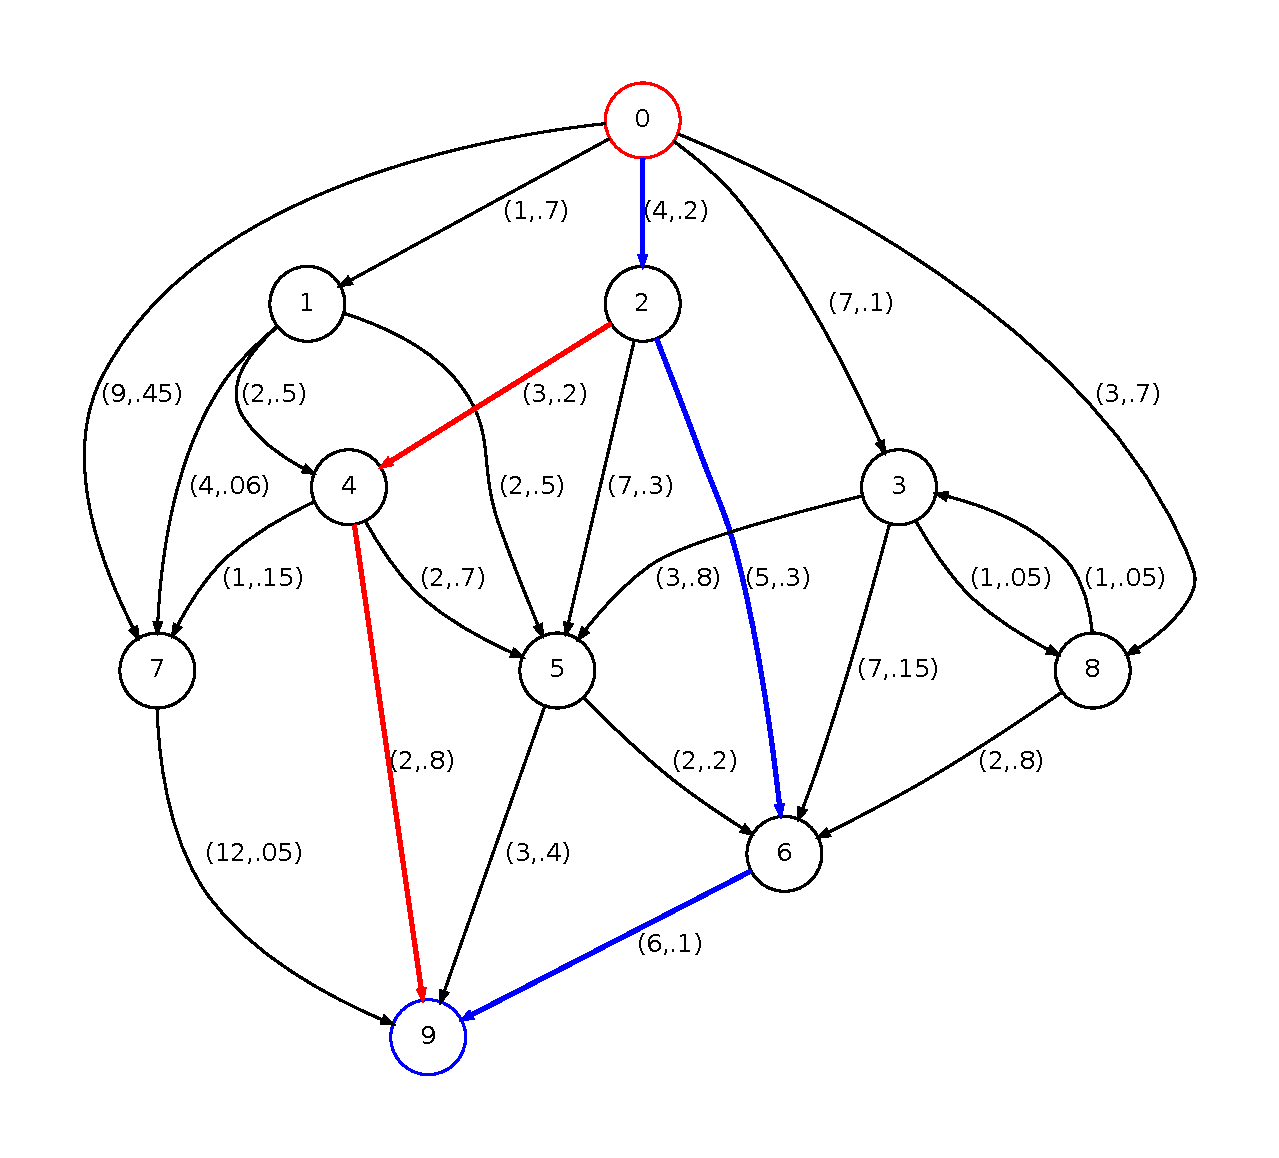
\includegraphics[scale=0.25]{fig/zang3a.pdf}
  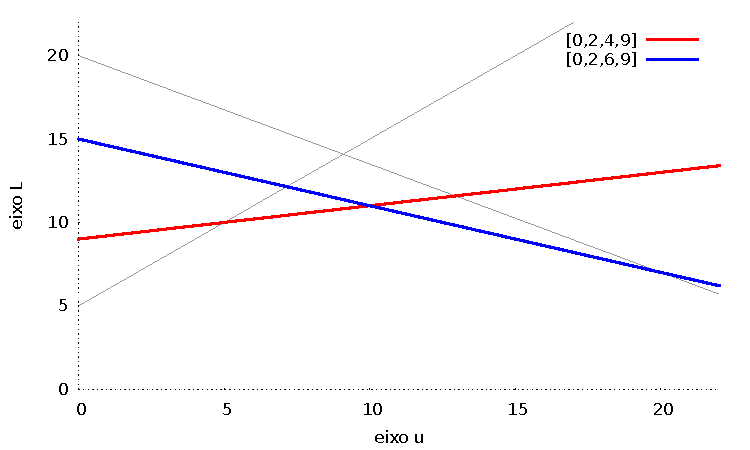
\includegraphics[scale=0.5]{fig/zang3b.pdf}
  \caption[Exemplo do algoritmo de Handler e Zang]{\tiny Avaliando a 
    função $L$ no ponto de interseção encontramos um caminho para 
    substituir $x^-$, a saber $[0,2,6,9]$. Agora na interseção de $x^+$ 
    e $x^-$ encontramos o ponto máximo da função $L$ que é $L^* = 11$ e 
    $u^* = 10$.  Terminamos o dual com $LB = 11$ e $UB = 15$.}
  \label{fig:zang1}
\end{figure}
}
\framet[Relaxação Lagrangiana]{
\begin{figure}[h!]
  \centering
  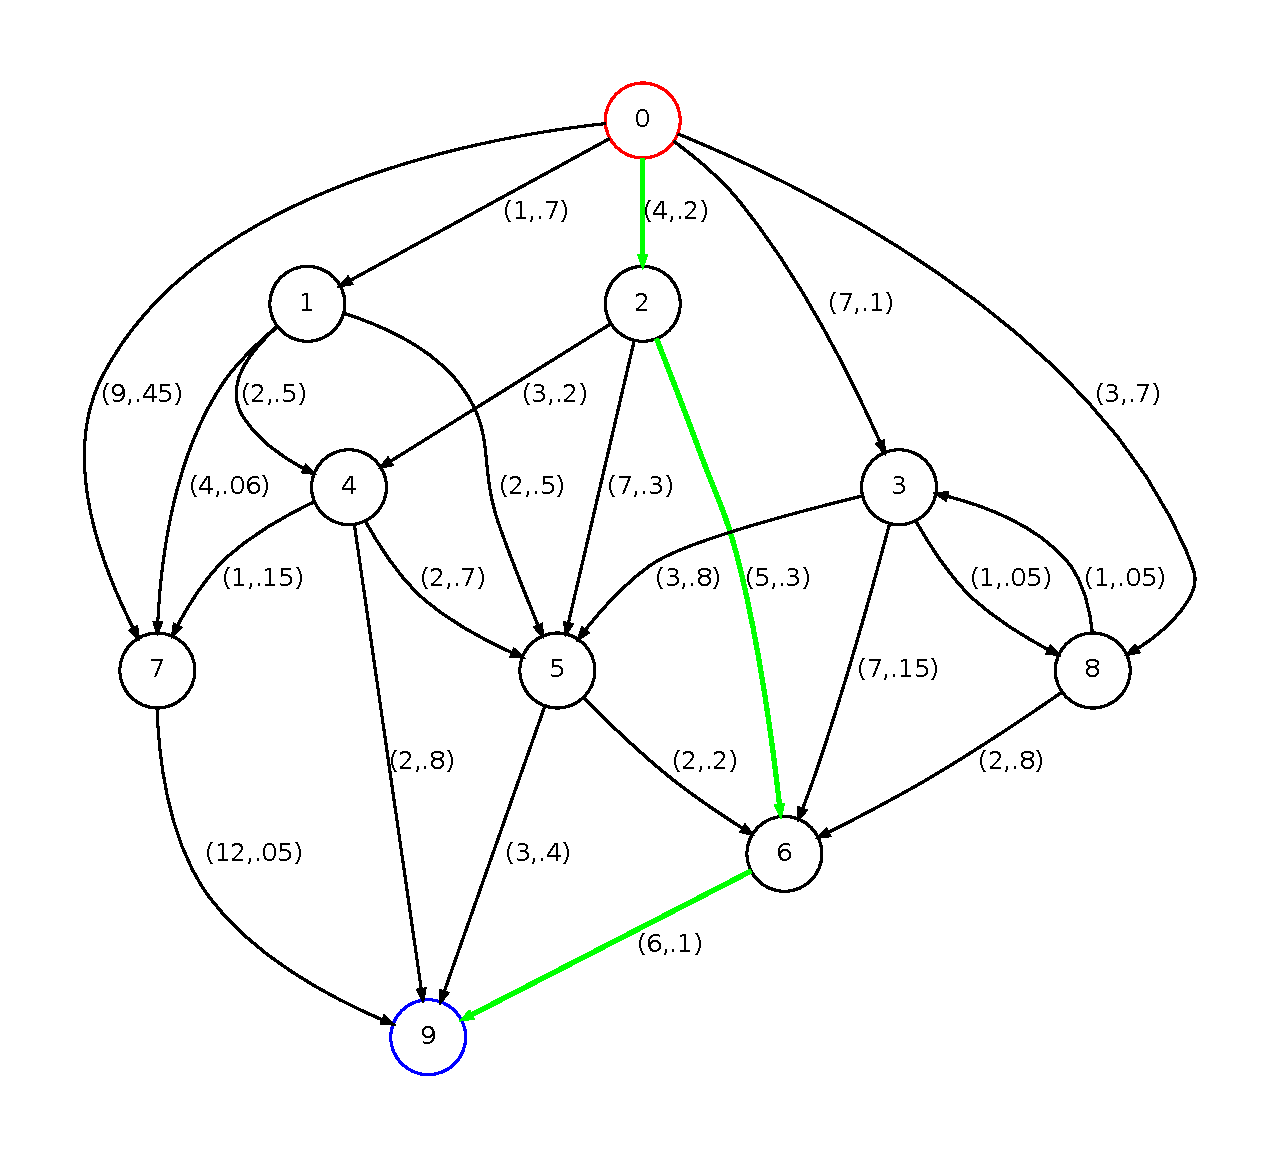
\includegraphics[scale=0.25]{fig/zang6a.pdf}
  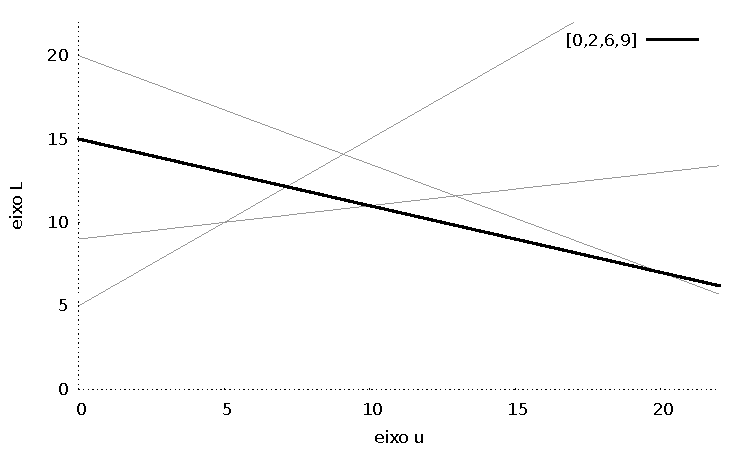
\includegraphics[scale=0.5]{fig/zang6b.pdf}
  \caption[Exemplo do algoritmo de Handler e Zang]{\tiny A partir daqui, 
  executamos o algortimo de Yen para eliminação da folga da dualidade.}
  \label{fig:zang1}
\end{figure}
}
\framet[Relaxação Lagrangiana]{
\begin{figure}[h!]
  \centering
  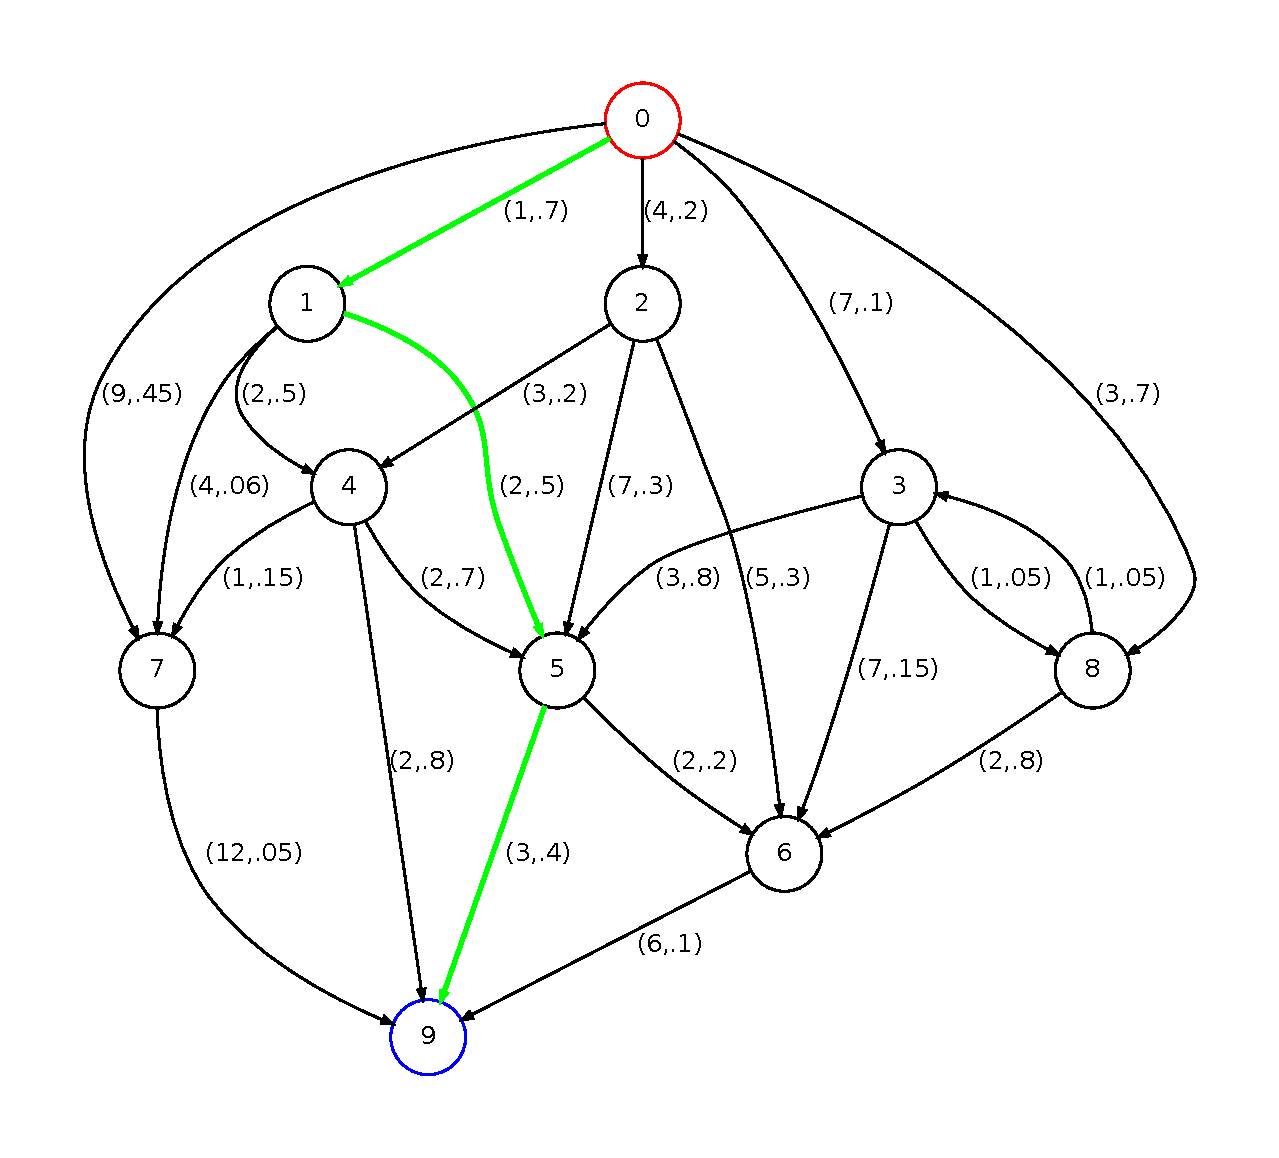
\includegraphics[scale=0.25]{fig/zang7a.pdf}
  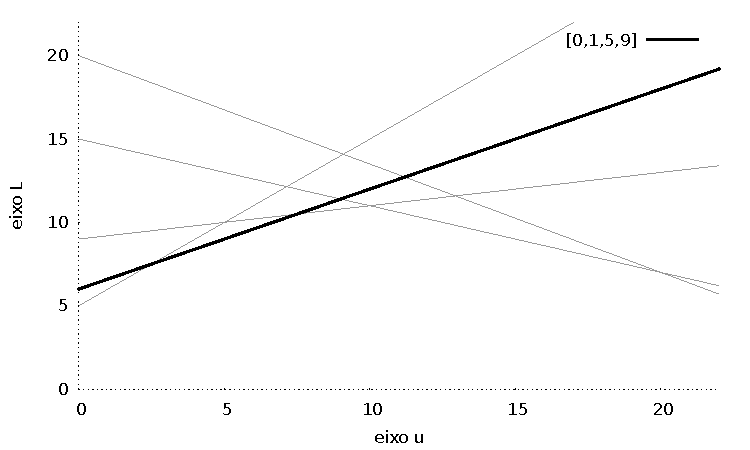
\includegraphics[scale=0.5]{fig/zang7b.pdf}
  \caption[Exemplo do algoritmo de Handler e Zang]{\tiny Eliminando a 
  folga da dualidade.}
  \label{fig:zang1}
\end{figure}
}
\framet[Relaxação Lagrangiana]{
\begin{figure}[h!]
  \centering
  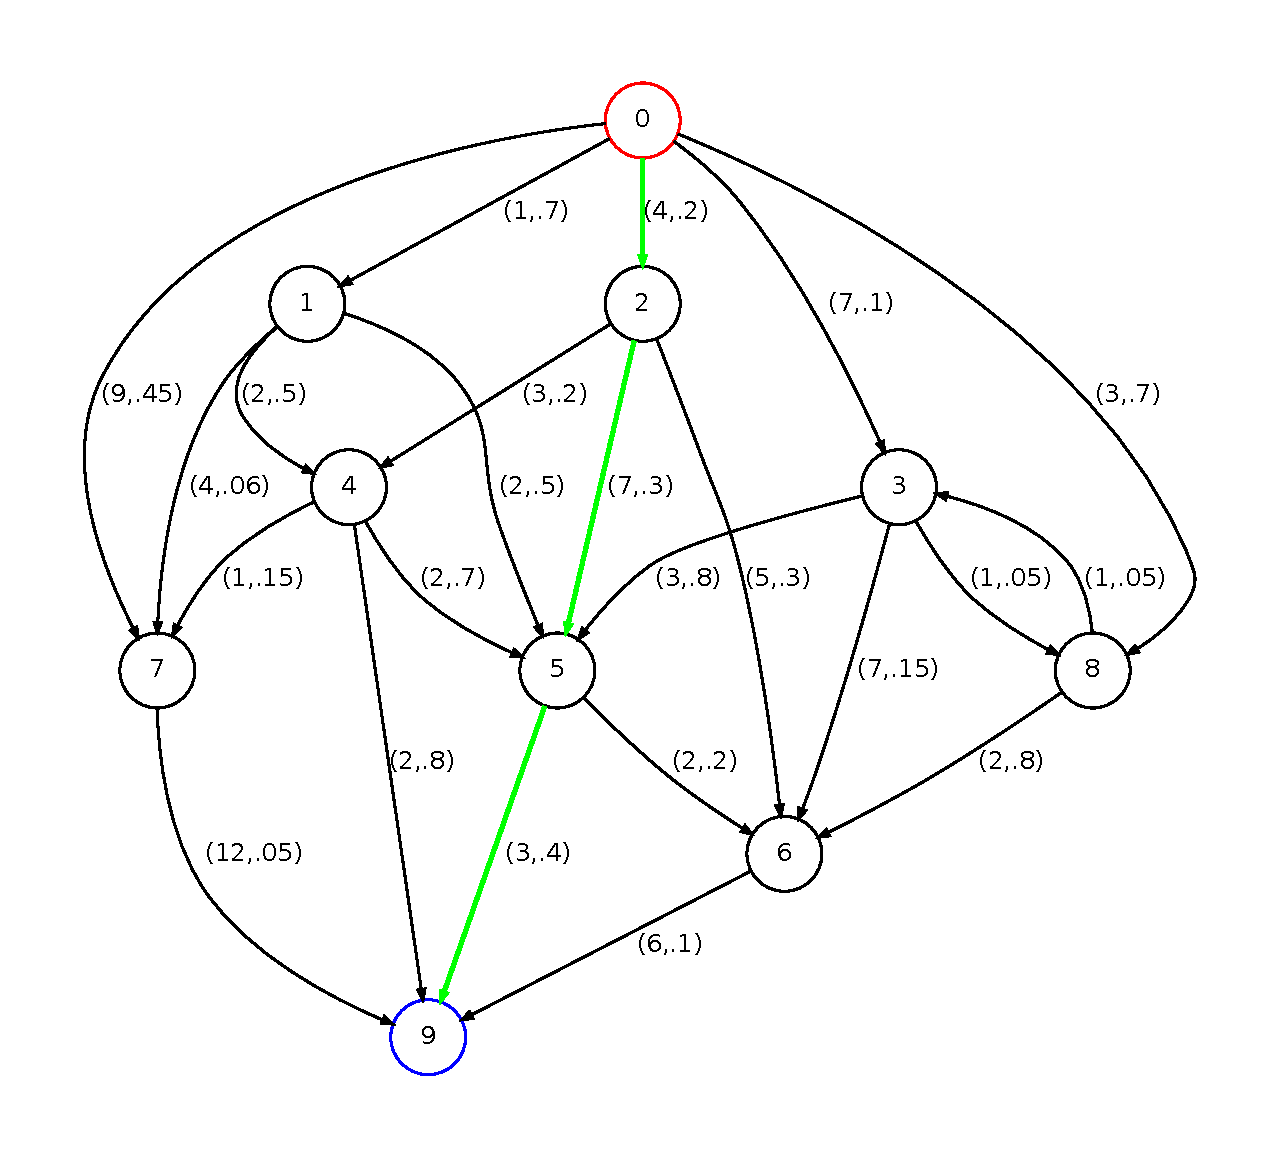
\includegraphics[scale=0.25]{fig/zang8a.pdf}
  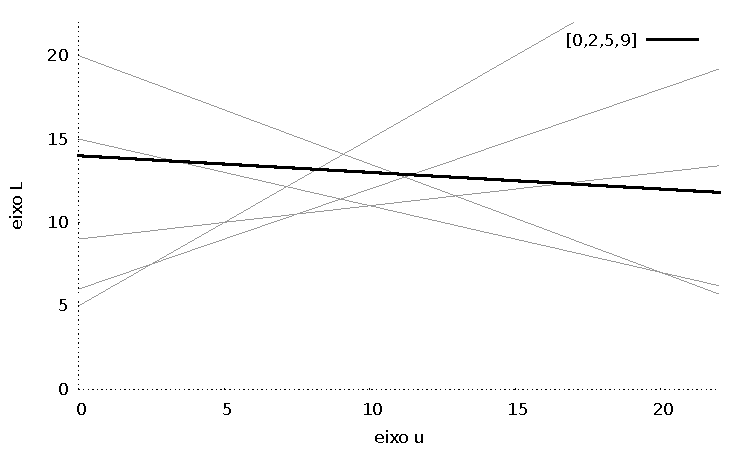
\includegraphics[scale=0.5]{fig/zang8b.pdf}
  \caption[Exemplo do algoritmo de Handler e Zang]{\tiny Eliminando a 
  folga da dualidade.}
  \label{fig:zang1}
\end{figure}
}
\framet[Relaxação Lagrangiana]{
\begin{figure}[h!]
  \centering
  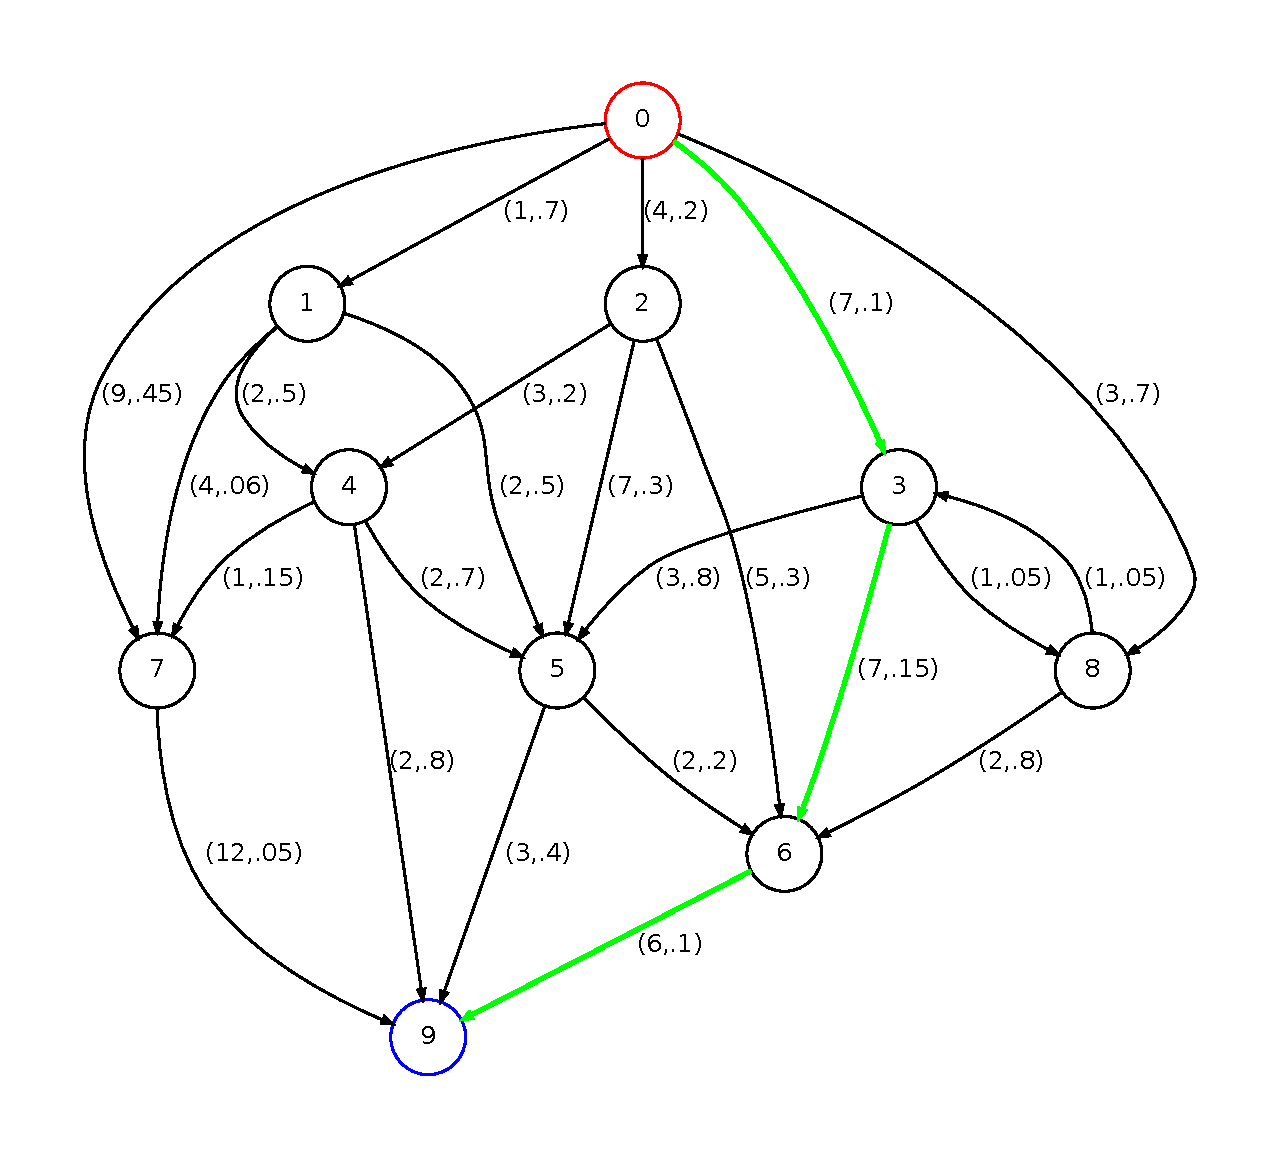
\includegraphics[scale=0.25]{fig/zang9a.pdf}
  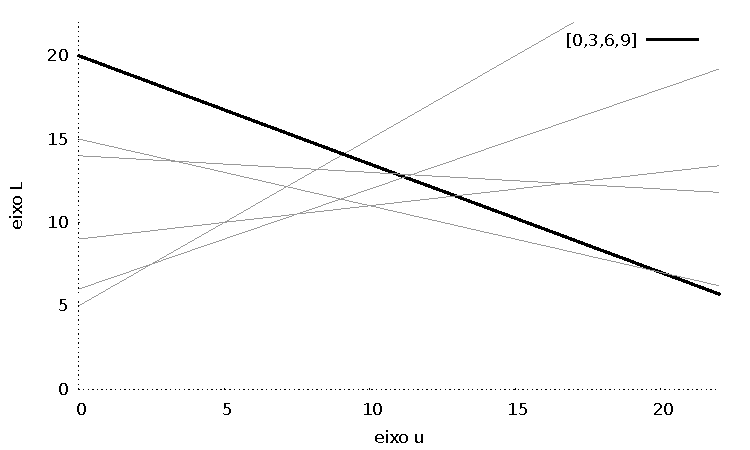
\includegraphics[scale=0.5]{fig/zang9b.pdf}
  \caption[Exemplo do algoritmo de Handler e Zang]{\tiny Eliminando a 
  folga da dualidade.}
  \label{fig:zang1}
\end{figure}
}
\framet[Relaxação Lagrangiana]{
\begin{figure}[h!]
  \centering
  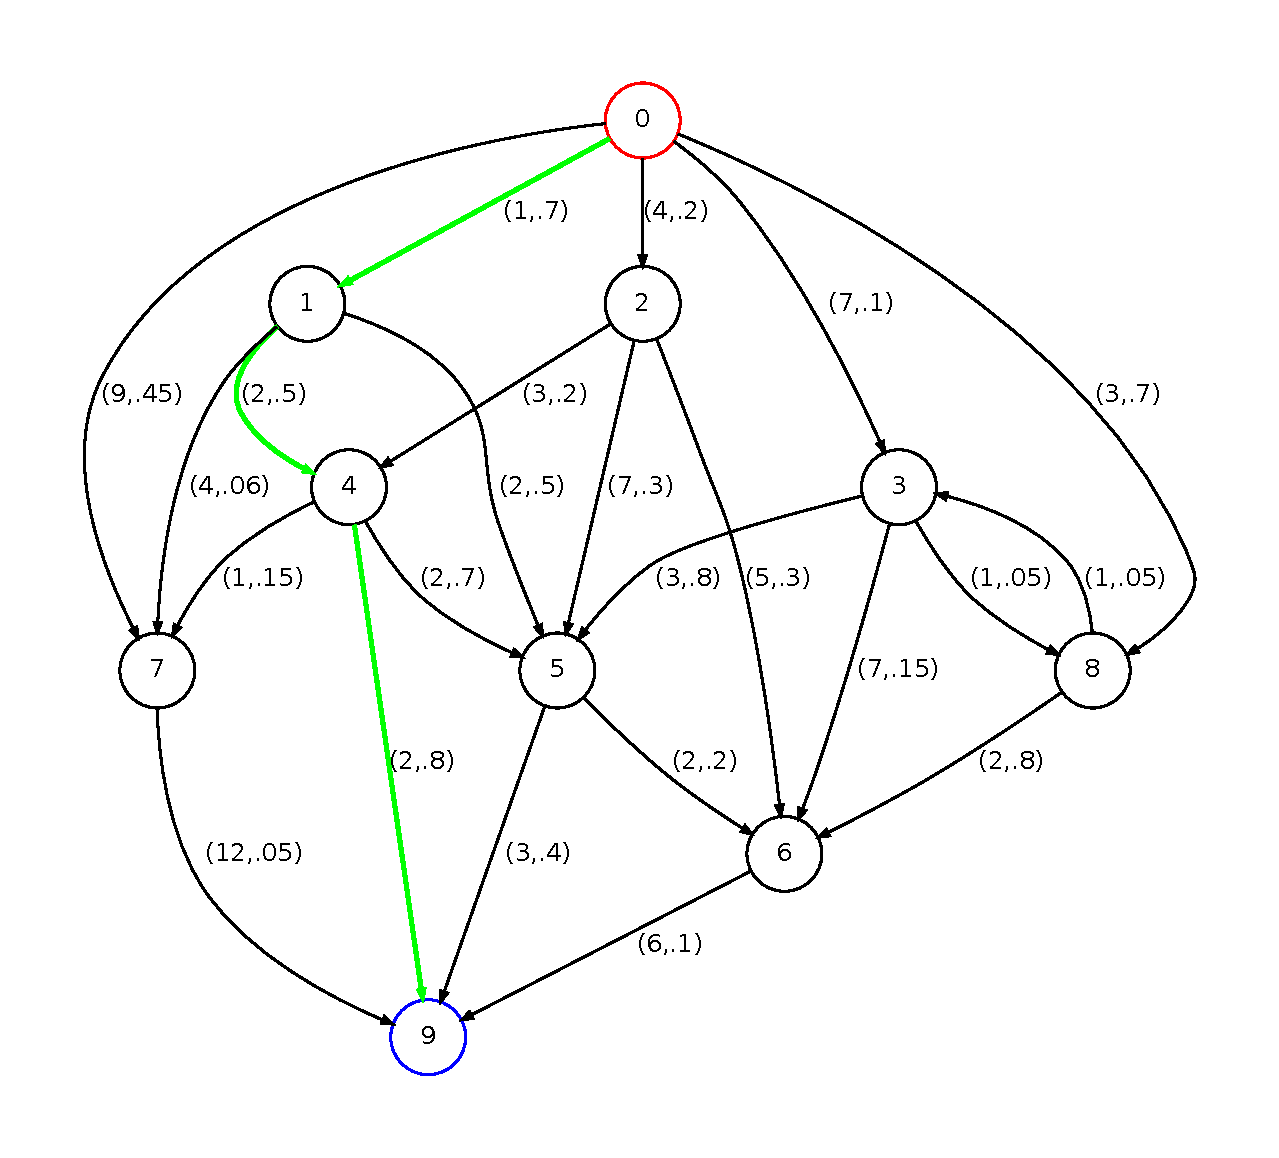
\includegraphics[scale=0.25]{fig/zang10a.pdf}
  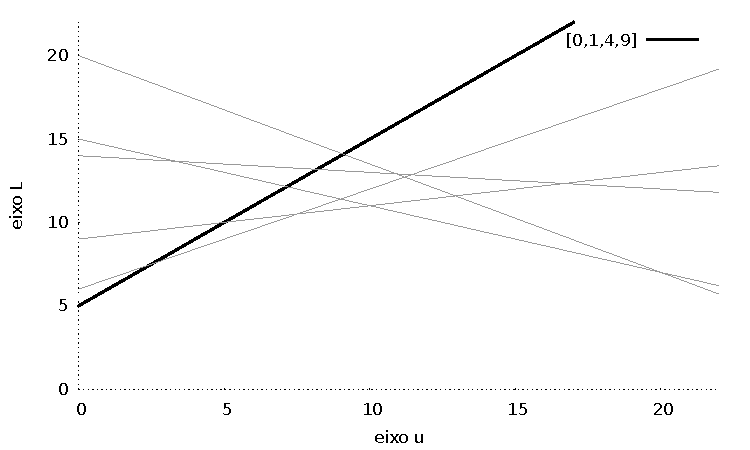
\includegraphics[scale=0.5]{fig/zang10b.pdf}
  \caption[Exemplo do algoritmo de Handler e Zang]{\tiny Eliminando a 
  folga da dualidade.}
  \label{fig:zang1}
\end{figure}
}
\framet[Relaxação Lagrangiana]{
\begin{figure}[h!]
  \centering
  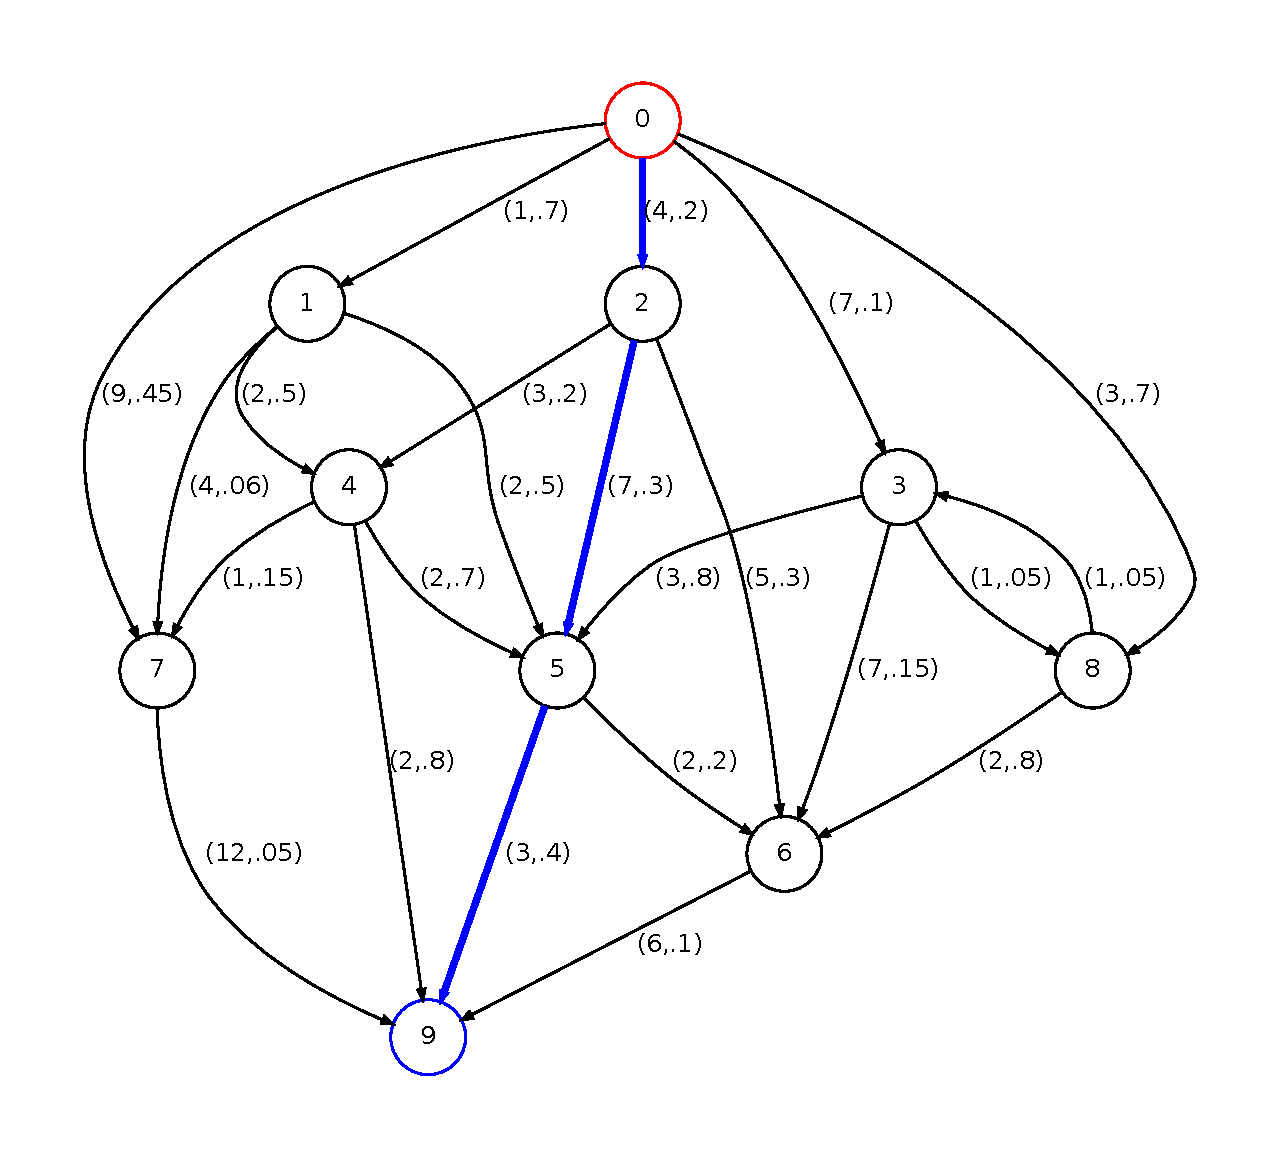
\includegraphics[scale=0.25]{fig/zang11a.pdf}
  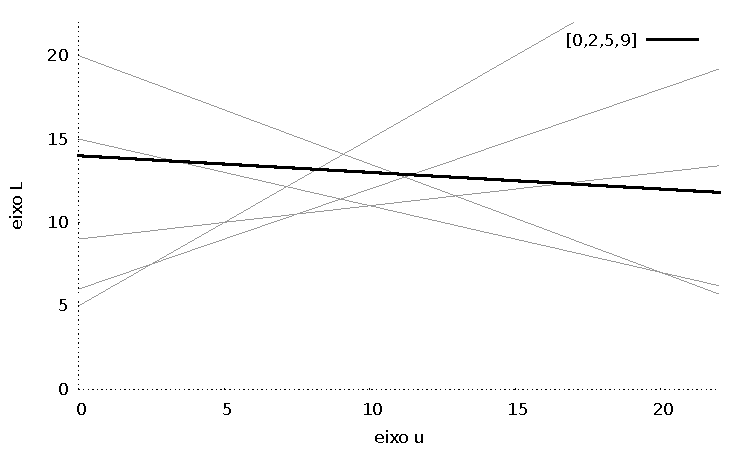
\includegraphics[scale=0.5]{fig/zang11b.pdf}
  \caption[Exemplo do algoritmo de Handler e Zang]{\tiny Solução 
  encontrada para o exemplo.}
  \label{fig:zang1}
\end{figure}
}

\section{Experimentos}
\stepcounter{subsection}

\framei[Ambiente computacional]{
\pause \item \emph{Laptop Sony Vaio},
\item com processador \emph{Intel Core i3 CPU M 330 @ 2.13GHz} e
\item $2$GB de memória RAM.
\item Sistema operacional Ubuntu (\emph{12.04 LTS 64 bit, kernel 
  3.2.0-27-generic}).
\item Implementações em C++ e
\item compilador g++ da GNU ($4.6.3$).

}


\framet[Dados de Teste] {
  \footnotesize
\textbf{DEM}: Modelos digitais de elevação (\emph{digital elevation 
models}) são grafos em forma de grade onde cada vértice tem um valor de 
altura associado. Estamos interessados em minimizar a diferença de 
altura acumulada no caminho com limitação do comprimento do caminho.  
Exemplos cedidos por Mark Ziegelmann (\cite{ziegelmann:01}). 

\begin{table}[ht!]
  \centering
  \begin{tabular}{|c|c|c|c|c|c|c|c|}
    \hline
    & Número de Vertices & Número de Arcos \\
    \hline
    Austria grande & 41600 & 165584 \\
    Austria pequeno & 11648 & 46160 \\
    \hline
  \end{tabular}
  \caption{\tiny Casos de teste do tipo \textbf{DEM}}
  \label{tab:testes_dem}
\end{table}

}

\framet[Dados de Teste] {
  \footnotesize
\textbf{ROAD}: Temos exemplo de grafos de ruas dos Estados Unidos 
fornecidos por Mark Ziegelmann. Congestionamento como função de custo.  
Nossa função custo é a distância euclidiana entre os pontos finais dos 
arcos. Estamos interessados em minimizar o congestionamento sujeito a um 
comprimento limitado.

\begin{table}[ht!]
  \centering
  \begin{tabular}{|c|c|c|c|c|c|c|c|}
    \hline
    & Número de Vertices & Número de Arcos \\
    \hline
    Road 1 & 77059 & 171536 \\
    Road 2 & 24086 & 50826 \\
    \hline
  \end{tabular}
  \caption{\tiny Casos de teste do tipo \defi{ROAD}}
  \label{tab:testes_road}
\end{table}
}


\framet[Dados de Teste] {

  \footnotesize
\defi{CURVE}: Temos exemplos de polígonos extraídos de mapas 
geográficos.  Assumindo que os pontos de quebra na curva dada ocorrem na 
ordem $v_1, v_2, \cdots, v_n$, nós usamos os pontos de quebra como 
vértices e adicionamos arcos $v_iv_j$ para cada $i < j$. 

\begin{table}[ht!]
  \centering
  \begin{tabular}{|c|c|c|c|c|c|c|}
    \hline
    & Número de Vertices & Número de Arcos \\
    \hline
    Curva 1 & 10000 & 99945 \\
    Curva 2 & 10000 & 199790 \\
    Curva 3 & 1000 & 9945 \\
    Curva 4 & 1000 & 19790 \\
    Curva 5 & 5000 & 49945 \\
    Curva 6 & 5000 & 99790 \\
    \hline
  \end{tabular}
  \caption{\tiny Casos de teste do tipo \textbf{CURVE}}
  \label{tab:testes_curve}
\end{table}



}


\framet[Dados de Teste] {
  \footnotesize
\defi{BC}: \citet{beasley:89} disponibilizaram $24$ casos de teste para 
o problema. Os dados foram gerados de forma randômica e contêm até $500$ 
vértices e $4800$ arcos. Para mais informações a respeito da forma de 
gerar os dados, recomendamos a leitura do artigo original.

\tiny
\begin{table}[ht!]
  \centering
  \begin{tabular}{|c|c|c|c|c|c|c|c|}
    \hline
    & Número de Vértices & Número de Arcos \\
    \hline
    1 & 100 & 955 \\
    2 & 100 & 955 \\
    3 & 100 & 959 \\
    4 & 100 & 959 \\
    5 & 100 & 990 \\
    6 & 100 & 990 \\
    7 & 100 & 999 \\
    8 & 100 & 999 \\
    9 & 200 & 2040\\
   10 & 200 & 2040\\
   11 & 200 & 1971\\
   12 & 200 & 1971\\
   13 & 200 & 2080\\
   14 & 200 & 2080\\
   15 & 200 & 1960\\
   16 & 200 & 1960\\
   17 & 500 & 4858\\
   18 & 500 & 4858\\
   %19 & 500 & 4978\\
   %20 & 500 & 4978\\
   %21 & 500 & 4847\\
   %22 & 500 & 4847\\
   %23 & 500 & 4868\\
   %24 & 500 & 4868\\
    \hline
  \end{tabular}
  \caption{\tiny Casos de teste do tipo \citet{beasley:89},}   
  \label{tab:testes_bc}
\end{table}
}


\framet[Resultados BC] {
  \tiny
\begin{table}[h!]
  \centering
  \begin{tabular}{|c|c|c|c|c|c|c|c|}
    \hline
    &PDP t(s)&PDP m(KB)&Yen t(s)&Yen m(KB)&
    HZ t(s)&HZ m(KB)\\
    \hline
    1 & 0.06 & 23248 & 0.01 & 6336&0.00&7088\\
    2 & 0.07 & 23248 & 0.02 & 6336&0.00&7072\\
    3 & 0.06 & 23152 & 0.01 & 6288&0.00&7056\\
    4 & 0.07 & 23152 & 0.02 & 6320&0.00&6656\\
    5 & 0.07 & 23376 & 0.01 & 6352&0.01&7104\\
    6 & 0.08 & 23344 & 0.01 & 6352&0.01&7104\\
    7 & 0.06 & 23168 & 0.01 & 6320&0.00&7088\\
    8 & 0.07 & 23168 & 0.01 & 6336&0.00&7088\\
    9 & 0.06 & 23264 & 0.08 & 6544&0.01&8496\\
   10 & 0.07 & 23264 & 0.08 & 6544&0.00&8512\\
   11 & 0.07 & 23312 & 0.01 & 6496&0.00&7456\\
   12 & 0.07 & 23296 & 0.02 & 6496&0.00&7456\\
   13 & 0.07 & 23376 & 0.02 & 7456&0.01&8304\\
   14 & 0.07 & 23360 & 0.02 & 7456&0.01&8320\\
   15 & 0.06 & 23312 & 0.02 & 6528&0.00&7456\\
   16 & 0.07 & 23296 & 0.02 & 6512&0.00&7456\\
   17 & 0.16 & 25120 & 0.03 & 9536&0.02&13296\\
   18 & 0.14 & 24928 & 0.04 & 9536&0.02&13296\\
   19 & 0.07 & 23728 & 0.04 & 9584&0.02&13408\\
   20 & 0.07 & 23696 & 0.05 & 9584&0.01&11296\\
   21 & 0.11 & 24272 & 0.04 & 9520&0.02&13280\\
   22 & 0.10 & 24208 & 0.04 & 9520&0.02&13280\\
   23 & 0.07 & 23680 & 0.04 & 9520&0.01&13360\\
   24 & 0.07 & 23696 & 0.04 & 9520&0.01&13344\\
    \hline
  \end{tabular}
  \caption{Tempo de execução para os testes \defi{BC}.}
\end{table}


}

\framet[Resultados BC] {
\begin{figure}[!h]
  \centering
  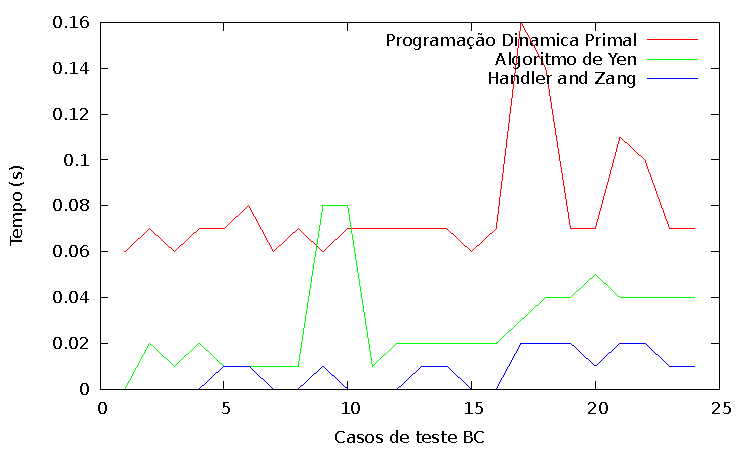
\includegraphics[scale=0.4]{fig/bc_tempo.pdf}
  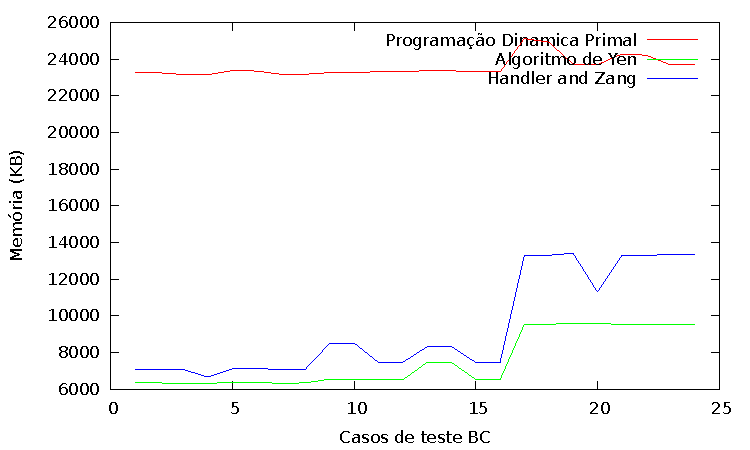
\includegraphics[scale=0.4]{fig/bc_memoria.pdf}
  \caption[Gráficos comparando consumo de memória e tempo dos algoritmo 
  de programação dinâmica primal, algoritmo de Yen e algoritmo de 
Handler e Zang.]{\tiny Gráficos comparando consumo de memória e tempo 
  dos algoritmo de programação dinâmica primal, algoritmo de Yen e 
algoritmo de Handler e Zang.} \label{fig:gps}
\end{figure}
}


\framet[Resultados DEM] {
  \footnotesize
\begin{table}[h!]
  \centering
  \begin{tabular}{|c|c|c|c|c|c|c|c|}
    \hline
    & HZ t(s) & HZ m(KB) & Iterações\\
    \hline
    Austria grande & 208.25 & 451440  & 169\\
   Austria pequeno & 7.66 & 119008 & 79\\
    \hline
  \end{tabular}
  \caption{\tiny Resultados dos casos de teste do tipo \textbf{DEM}}
  \label{tab:resultados_dem}
\end{table}
}

\framet[Resultados ROAD] {
  \footnotesize
\begin{table}[h!]
  \centering
  \begin{tabular}{|c|c|c|c|c|c|c|c|}
    \hline
    & HZ t(s) & HZ m(kb) & Iterações\\
    \hline
    Road 1 & 853.88 & 1303264 & 1258\\
    Road 2 & 12.52 & 189072 & 214\\
    \hline
  \end{tabular}
  \caption{\tiny Resultados dos casos de teste do tipo \defi{ROAD}}
  \label{tab:resultados_road}
\end{table}
}

\framet[Resultados CURVE] {
  \footnotesize
\begin{table}[h!]
  \centering
  \begin{tabular}{|c|c|c|c|c|c|c|}
    \hline
    & HZ t(s) & HZ m(KB) & HZ Iterações & DPP t(s) & DPP m(KB)\\
    \hline
    Curva 1 & 1.76 & 163648 & 12 & 7.62 & 10280116 \\
    Curva 2 & 80.83 & 718560 & 22 & 12.51 & 1100832 \\
    Curva 3 & 0.08 & 20928 & 8 & 0.07 & 27264 \\
    Curva 4 & 0.94 & 49888 & 15 & 0.14 & 35104 \\
    Curva 5 & 28.56 & 629776 & 110 & 1.48 & 234832 \\
    Curva 6 & 1.15 & 154368 & 11 & 2.47 & 270528 \\
    \hline
  \end{tabular}
  \caption{\tiny Resultados dos casos de teste do tipo \textbf{CURVE}}
  \label{tab:resultados_curve}
\end{table}
}

\framet[Resultados CURVE] {
\begin{figure}[!h]
  \centering
  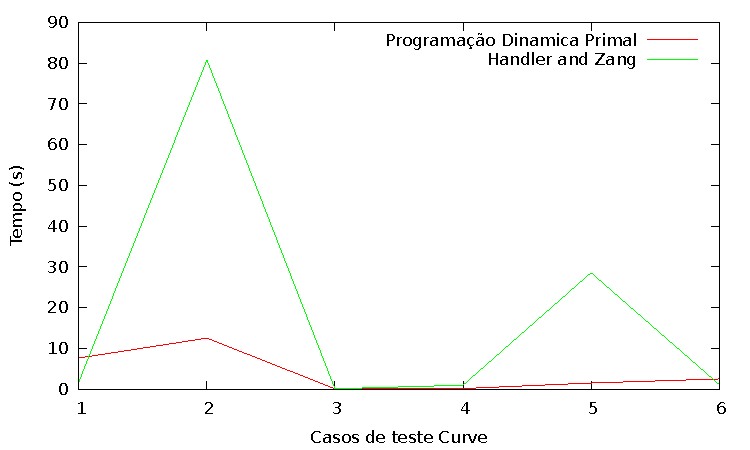
\includegraphics[scale=0.4]{fig/curva_tempo.pdf}
  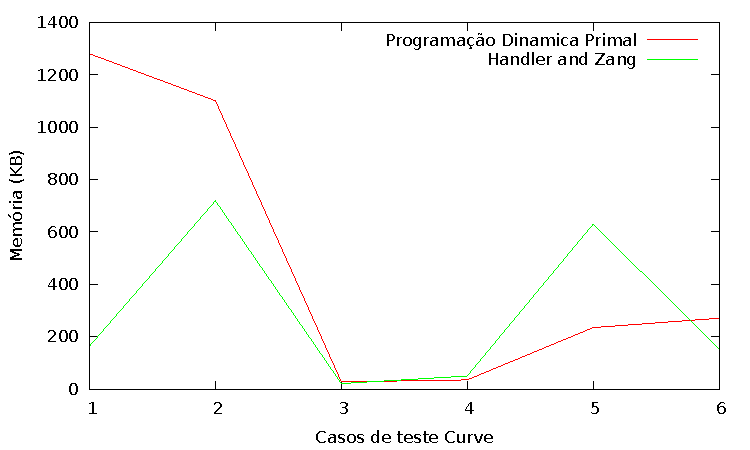
\includegraphics[scale=0.4]{fig/curva_memoria.pdf}
  \caption[Gráficos comparando consumo de memória e tempo dos algoritmo 
  de programação dinâmica primal e algoritmo de Handler e Zang.]{\tiny 
  Gráficos comparando consumo de memória e tempo dos algoritmo de 
programação dinâmica primal Yen e algoritmo de Handler e Zang para os 
casos do tipo de curva de aproximação.} \label{fig:rescurva}
\end{figure}
}

%\framet[Kaggle] {
    %\fig[1]{kaggleconvergenceen}{Curva de convergência de uma 
    %competição no Kaggle}
%}

%\framet[Joone - Sinapses] {
    %\begin{figure}[!ht]
        %\centering
        %\subfigure[DirectSynapse]
        %{
            %\includegraphics[width=0.45\textwidth]{fig/directsynapse} }
        %\subfigure[FullSynapse]
        %{
            %\includegraphics[width=0.44\textwidth]{fig/fullsynapse}
        %}
    %\end{figure}
%}


%\normalsize
%\begin{block}{}
    %A arquitetura de Jordan apresentou melhores resultados na média 
    %para
    %um maior número de séries.
%\end{block}

%\section{Referências}
\stepcounter{subsection}
\begin{frame}[allowframebreaks]
  %\frametitle{Referências}
  \tiny
  \bibliographystyle{plainnat-ime} % citação bibliográfica textual
  \bibliography{references}
\end{frame}

\frame{
  \hfill \begin{center} Obrigado!\\joelsu@ime.usp.br \end{center} \hfill
}

\end{document}
